\documentclass[a4paper,11pt]{report}
\usepackage{geometry}      
\usepackage{multicol,float}         
\usepackage{capt-of} 
\usepackage{booktabs}
\usepackage{siunitx}
\edef\oldtt{\ttdefault}
\usepackage[scaled]{beramono}
\usepackage[T1]{fontenc}
\renewcommand{\ttdefault}{\oldtt}
\newcommand{\bera}[1]{{\fontfamily{fvm}\selectfont \blue{#1}}}
\geometry{a4paper,left=2cm,right=2.5cm,top=2.5cm,bottom=2.5cm}                 % ... or a4paper or a5paper or ... 
\usepackage{graphicx}
% tikz 画图 宏包
\usepackage{tikz}
\usepackage{circuitikz}

\usepackage{subfigure} % 多图并列
\usetikzlibrary{intersections}
\usetikzlibrary{shapes,arrows,positioning}
\usepackage{amsmath, amssymb}
\usepackage{enumerate}
\usepackage{wrapfig}
% \usepackage{subcaption}

\setlength\columnsep{0.8cm} %双栏间距长度 
\usetikzlibrary{shapes.geometric, arrows}

% 英文:自定义 定义、定理、引理 相关命令
\usepackage{amsthm}
\newtheorem{myDef}{Def}[section]
\newtheorem{myTheo}{Theorem}
\newtheorem{myle}{Lemma}
\newtheorem*{mypro}{证明}
% \newtheorem{example}{例}[section]
\newtheorem{example}{Example}[section]

\usepackage{enumitem}
% 支持中文
% \usepackage[UTF8]{ctex}

%行间距
\renewcommand{\baselinestretch}{1}
%段间距

%设置图片文件夹
\usepackage{graphicx}
\graphicspath{{./img/}}

% 设置字体
\usepackage{fontspec,xltxtra,xunicode}
\defaultfontfeatures{Mapping=tex-text}
\setromanfont[Mapping=tex-text]{Times New Roman}
\setsansfont[Scale=MatchLowercase,Mapping=tex-text]{Times New Roman}
% \setmonofont[Scale=MatchLowercase]{}

% 命令定义
\def\dis{\mathop{}\!\displaystyle}

\def\dif{\mathop{}\!\mathrm{d}}
\def\Var{\mathop{}\!\mathrm{Var \:}}

\def\sh{\mathop{}\!\mathrm{sh \:}}
\def\ch{\mathop{}\!\mathrm{ch \:}}
\def\thx{\mathop{}\!\mathrm{th \:}}
\def\arsh{\mathop{}\!\mathrm{arsh \:}}
\def\arch{\mathop{}\!\mathrm{arch \:}}
\def\arth{\mathop{}\!\mathrm{arth \:}}
\def\arccot{\mathop{}\!\mathrm{arccot \:}}
% \title{Microeconomics Note}
% \author{Michael Lea}

% \setlist[enumerate]{label=(\arabic*)}
% 修改 chapter section 等 title 的命令形式
\usepackage{titlesec}%chapter1修改为第1章
\renewcommand{\thechapter}{\Roman{chapter}}
\titleformat{\chapter}[hang]
  {\normalfont\large\centering}{\thechapter. }{0em}{\large}
\titlespacing*{\chapter}{0pt}{2em}{1em}

% % 重定义 section 的编号为大写字母
\renewcommand{\thesection}{\arabic{chapter}.\arabic{section}}
\titleformat{\section}
{\normalfont\normalsize\itshape}
{\arabic{chapter}.\arabic{section} }
{0em}
{}
\titlespacing*{\section}{0pt}{1.2em}{0.5em}

\renewcommand{\thesubsection}{\arabic{chapter}.\arabic{section}.\arabic{subsection}}
\titleformat{\subsection}
{\normalfont\normalsize\itshape}
{\arabic{chapter}.\arabic{section}.\arabic{subsection} }
{0em}
{}
\titlespacing*{\subsection}{0pt}{1em}{0.5em}


\usetikzlibrary {calc}

% 页码设计
\usepackage{lastpage}%获得总页数
\usepackage{fancyhdr}
\pagestyle{fancy}
\fancyhead[C]{Machine Learning}
\fancyhead[L]{Li Yihai - 23345919}
\fancyhead[R]{Final Assignment}

%以下命令中L--左侧 R--右侧 C--中间 O--奇数页 E--偶数页
% \fancyhead[LO,RE]{}%奇数页左侧,偶数页右侧显示页眉
\fancyfoot[CO,RE]{}%奇数页中间,偶数页右侧页脚为空
\fancyfoot[LO,CE]{}%奇数页左侧,偶数页中间页脚为空
\fancyfoot[CO,CE]{\thepage}%奇数页右侧,偶数页左侧显示 当前页 of 总页数
\renewcommand{\headrulewidth}{0.4pt}%改为0pt即可去掉页眉下面的横线
\renewcommand{\footrulewidth}{0.4pt}%改为0pt即可去掉页脚上面的横线


% Paragraph
\titleformat{\paragraph}[runin]
{\normalsize\itshape}{\theparagraph}{1em}{}

\newcounter{question}
\setcounter{question}{1}
\renewcommand{\thequestion}{\noindent\arabic{question}. }

% Equation
% \renewcommand{\theequation}{\footnotesize \thechapter.\arabic{equation}}
\renewcommand{\theequation}{\footnotesize \arabic{chapter}.\arabic{equation}}


% 设置图片caption的样式
\usepackage{hyperref}
\usepackage{caption}
\captionsetup[table]{width=.45\textwidth, labelsep=period}

\counterwithout{figure}{chapter}
\renewcommand{\figurename}{}
\captionsetup[figure]{width=0.45\textwidth, labelsep=period}
\renewcommand{\thefigure}{\normalsize{F}\footnotesize\text{ig \normalsize\arabic{figure}}}
\renewcommand{\figureautorefname}{Fig.}

\counterwithout{table}{chapter}
\renewcommand{\tablename}{}
\renewcommand{\thetable}{{\normalsize{T}\footnotesize\text{ABLE} \normalsize\Roman{table}}}

% 行间距
\setlength{\arraycolsep}{6pt} 
\renewcommand{\arraystretch}{1.3} 

\usepackage{listings}

% 用来设置附录中代码的样式
\usepackage{xpatch}
\makeatletter
\xpatchcmd{\chapter}
  {\if@openright\cleardoublepage\else\clearpage\fi}{\par\relax}
  {}{}
\makeatother

\usepackage{blindtext}
\usepackage{xcolor} % 如果尚未导入
\definecolor{darkgreen}{rgb}{0.0, 0.5, 0.0}
\lstdefinestyle{PythonStyle}{
    language=Python,             
    basicstyle=\ttfamily\footnotesize,  % 更新字体大小
    keywordstyle=\color{blue},   
    stringstyle=\color{orange},  
    commentstyle=\color{darkgreen},  
    morecomment=[s][\color{brown}]{"""}{"""},
    breaklines=true,             
    numbers=left,                
    numberstyle=\tiny\color{gray}, % 保持行号的字体为 \tiny
    showstringspaces=false,      
    frame=tb,                    
}

\lstdefinestyle{CStyle}{
    language=C,                  
    basicstyle=\ttfamily\footnotesize,  % 更新字体大小
    keywordstyle=\color{blue},   
    stringstyle=\color{orange},  
    commentstyle=\color{darkgreen},  
    breaklines=true,             
    numbers=left,                
    numberstyle=\tiny\color{gray}, % 保持行号的字体为 \tiny
    showstringspaces=false,      
    frame=tb,                    
}


\newcommand{\red}[1]{{\color{red}{#1}}}
\newcommand{\blue}[1]{{\color{blue}{#1}}}
\newenvironment{Figure}
  {\par\medskip\noindent\minipage{\linewidth}}
  {\endminipage\par\medskip}


\usepackage{pdfpages}
\usepackage{pdflscape}


\title{Stochastic Methods Homework}
\author{Li Yihai, 23345919}
\date{Assignment 3}


\begin{document}

% \maketitle
% \includepdf{chap/hw2_23-24.pdf}
{
  \begin{center}
    \Huge Dublin Bike-usage Assessment of Pandemic by Means of Deep Learning
  \end{center}
}
\vspace*{1em}
\begin{multicols}{2}
  \begin{center}
    Li Yihai \\
    Trinity College Dublin (TCD)\\
    School of Mathematics\\
    Student ID: 23345919 \\
    Module Code: CS7CS4 \\
    Assignment: Final
  \end{center}
\end{multicols}
\vspace*{2em}

\begin{multicols}{2}
% {
%     \bfseries
%     % \footnotesize
%     \noindent 
%     {
%         \itshape
%         Abstract
%     }.
%     As Dublin City Council asked to study the impact of 
%     COVID-19 on the city-bikes usage as they are planning 
%     to optimize city-bike system. This paper is the 
%     first step that is to investigate the impact of pandemic on the 
%     usage of the city bike network.
%     However, since the limitation of this paper is restricted into 8 papers 
%     and the limited machine tools. 
%     This paper 
%     selected features 
%     (\blue{'station id', 'time', 'bike stands', 'available bike stands', 'available bikes'}) 
%     which is useful for analyzing bike-usage from 
%     the full dataset published by Dublin City Council 
%     \cite{CityBikedataset}.  
%     Moreover, doing more feature engineering to these five features which ultimately 
%     became a time series with one feature of totally 118 bike stations. 
%     By using the regression models introduced in lectures, which are 
%     Ridge and Lasso regression models, this paper 
%     firstly applying $k$-fold cross validation to them on a 
%     sampled dataset. 
%     Considering the Long-Short Term Memory (LSTM) Recurrent Neural Networks (RNNs) 
%     are designed for 
%     handling time series, this paper began with introducing the 
%     concepts of RNNs and the LSTM. 
%     Then applied cross validation to a simple LSTM RNN model, compare
%     with regression models together. 
     

%     \noindent Keywords. Dublin City Bike-usage; Pandemic; Regression Models; Ridge; Lasso; Recurrent Neural Networks (RNNs);
%     Long-Short Term Memory (LSTM)
%     \vspace*{2em}
% }
\chapter{P\normalsize{REPROCESSING}}    
\section{Loading Data Files}
\paragraph{Raw Data}
Row data \cite{CityBikedataset} are included in 41 files, staring from the 2018-10-01 to 
2023-12-25. They included information of Dublin-bikes, in features 
:\blue{ 'station id', 'time', 'last updated', 'name', 'bike stands',
'avaliable bike stands', 'avaliable bikes', 'status', 'address',
'latitude', 'longitude'} for 118 stations in Dublin city. 
% The table below is a demo of row data files

\begin{figure}[H]
    \centering
    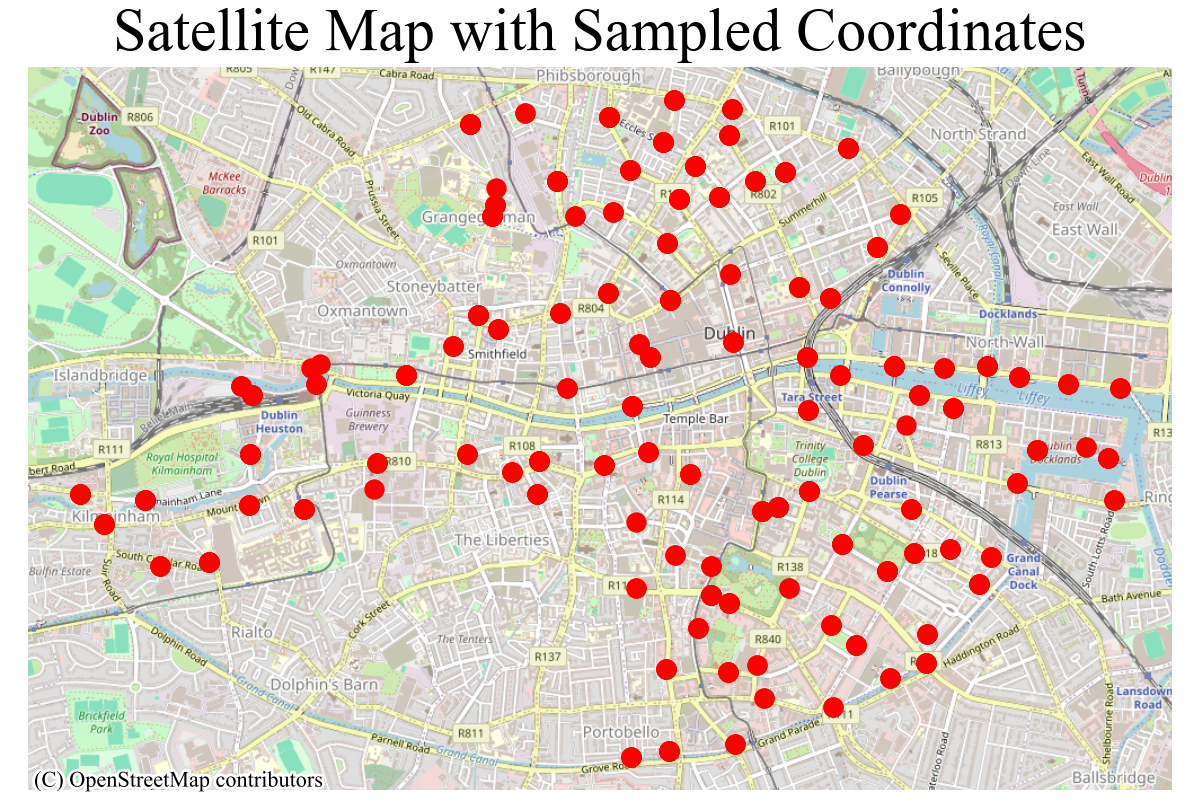
\includegraphics[width=0.45\textwidth]{chap/fig0.png}
    \caption{
        \footnotesize
        Satellite coordinates of bike stations
        } % 表格标题
    \label{FIGURES: CORRD}
\end{figure}

\paragraph{Data Spliting}
In order to handle the tasks, the row data required to be preprocessed before 
staring analysis them. Since the main tasks are assess the impact of the 
pandemic on the city-bike usage, the data files are divided into three parts 
by the time stamps of beginning of city-school were closed 
\cite{OHalloran2020Pandemic} and the 
HSE stopped releasing pandemic figures \cite{OHalloran2022Pandemic}. 
Respectively, the data files 
are stand for before, during and post pandemic periods.

\paragraph{Data Cleaning} 
Besides that, there are two type of features in the files where the one stands for 
city-bike usage and the other one stands for the information of each bike station.
Thus, there will be additional data file for storing the information of all stations 
including \blue{ 'station id', 'name', 'address', 'latitude', 'longitude'}.
Treat the missing values as 0 for all values and delete the repeated sample values.

\paragraph{Rounding}
Considering the pandemic was continued for years and the data were sampling in few 
seconds which is unnecessary for analyzing the general pattern in the large picture 
across years. Thus, excluding load and split raw data files, rounding the 
time stamps to nearest 8 hours and determine the mean of each feature values in 
that 8 hours. Such procedure could reduce the demanding of computation resources and 
make it easier to find general pattern.

\section{Feature Engineering}
\paragraph{Modify Features}
According to the hints, the "bike usage" can be represented by the number of 
bikes have been taken from (or brought to) that station.
The features that can might be use to tasks are 
\blue{'station id', 'time', 'bike stands', 'available bike stands', 'available bikes'}.

Moreover, for a station, the number of available bike stands and available bikes can 
determine the value of total bike stands which is the sumption of them. 
However, available bike stands $(N_{stands}(t))$ and bikes $(N_{bikes}(t))$ 
at some time stamps $(t)$ do not show the usage of bikes. 

In order to solving this problem without 
applying complicate methods, 
define the difference of $N_{stands}(t)$ 
and $N_{bikes}(t)$ as $N_{\text{bring stand bikes}}(t) $ and 
$N_{\text{take bikes}}(t) $ where follow
\[
    \begin{cases}
        N_{\text{bring stand bikes}}(t) 
        = 
        N_{\text{stands}}(t-\Delta t) 
        - 
        N_{\text{stands}}(t) \\
        N_{\text{take bikes}}(t) 
        = 
        N_{\text{bikes}}(t-\Delta t) 
        - 
        N_{\text{bikes}}(t)
    \end{cases}
\]
For $N_{\text{bring stand bikes}}(t)$,
it means that 
there are $N_{\text{bring stand bikes}}(t)$ bike stands 
get a returned bike in 
time interval $[t, t+\Delta]$.
The other $N_{\text{bikes}}(t)$ means that there are
$N_{\text{take bikes}}(t)$ bikes are brought in 
time interval $[t, t+\Delta]$.
After that, 
\[
N_{\text{bring stand bikes}}(t)  + N_{\text{take bikes}}(t) 
\]
the number of bike were using by citizens.
Theoretically, the sumption 
$
N_{\text{bring stand bikes}}(t)  + N_{\text{take bikes}}(t) 
$ equals to $0$
as long as no bikes are used.
At the end of processing, $Z$-score normalize the $3$ separated data files
separately, which make shift the mean of data to $0$ and the 
standard deviation to $1$.
It follows 
\[
    Z = \frac{X - \mu}{\sigma}
\]
where the $X$ is original data and $\mu$, $\sigma$ are mean and 
standard deviation of original data.

Overall, the feature: \blue{'using bikes'} in time interval $[t, t+\Delta]$ are 
\[
    N_{\text{using bikes}}(t) = N_{\text{bring stand bikes}}(t)  +  2N_{\text{take bikes}}(t) 
\]
where the $\Delta = 8$ (hour). It means that there are $N_{\text{using bikes}}(t)$
bikes are used for the station between $t$ and $t+8$ (hour). 
The data with $N$ samples can be formulated as  
\[
   \left\{(t_k, y_k)\right\}_{k = 0}^{N}
\]where $t_k$ is the time of $k^{\text{th}}$ the measurement and 
$y_k$ is the $k$ measurement of \blue{using bikes} in $\left[t_k, t_{k+1}\right]$.

\paragraph{Feature Engineering for Times Series}\label{sec:FeatureEngineerforTimeSeries}
Time series features data has many compositions, it includes 
trends, seasonality, and irregular variations in 
stations analysis. 
The prediction model $\widehat{f}_d$ uses $n$ continues samples to predict 
$q$ step ahead every $d$ time stamp which means 
\[
    \widehat{y}_{k+q} = \widehat{f}_d(y_{k-nd}, y_{k-nd+d}, \cdots, y_{k-d})
\] 
Since various $d$ represent predicting using different cycility, thus using
a combination of $\widehat{f}_d$ to
predict on cycility $d_0,d_1, \cdots, d_m$. Collectively, the prediction model follows
% \[
%     \widehat{y}_{k+q} = 
%     \widehat{f}
%     (y_{k-nd_0}, y_{k-nd_0+d_0}, \cdots, y_{k-d_0}, 
%     \cdots,
%     y_{k-nd_s}, y_{k-nd_s+d_s}, \cdots, y_{k-d_s})
% \]
\begin{align*}
    \widehat{y}_{k+q} = 
    \widehat{f}
    (&y_{k-nd_0}, y_{k-nd_0+d_0}, \cdots, y_{k-d_0}, 
    \\ &\cdots,\\
    &y_{k-nd_s}, y_{k-nd_s+d_s}, \cdots, y_{k-d_s})
\end{align*}
where the parameters $q$, $n$ and $d_0,d_1, \cdots, d_s$ are hyperparameters. 
The processed dataset $y$ has shape
\[
    \left(
        N-(n+1)\max_{i = 0}^{s}
        N_i -q
        , 
        ns
        \right)
\]
where $N_i$ is the number of samples in $d_i$ cycility.
More specific features engineering will be discussed with model designs.

\section{Visualization}
In this part, visualize the bike-usage data in pandemic period of the 
station $3$ and $4$. 
The points at positive region in the \ref{FIGURES: FEATURED DATA} 
mean the bike was took in the at the time step. 
On the contrast, negative value mean the bike was returned bike to station, and 
$0$ means no bike-usage at the time step.
\begin{figure}[H]
    \centering
    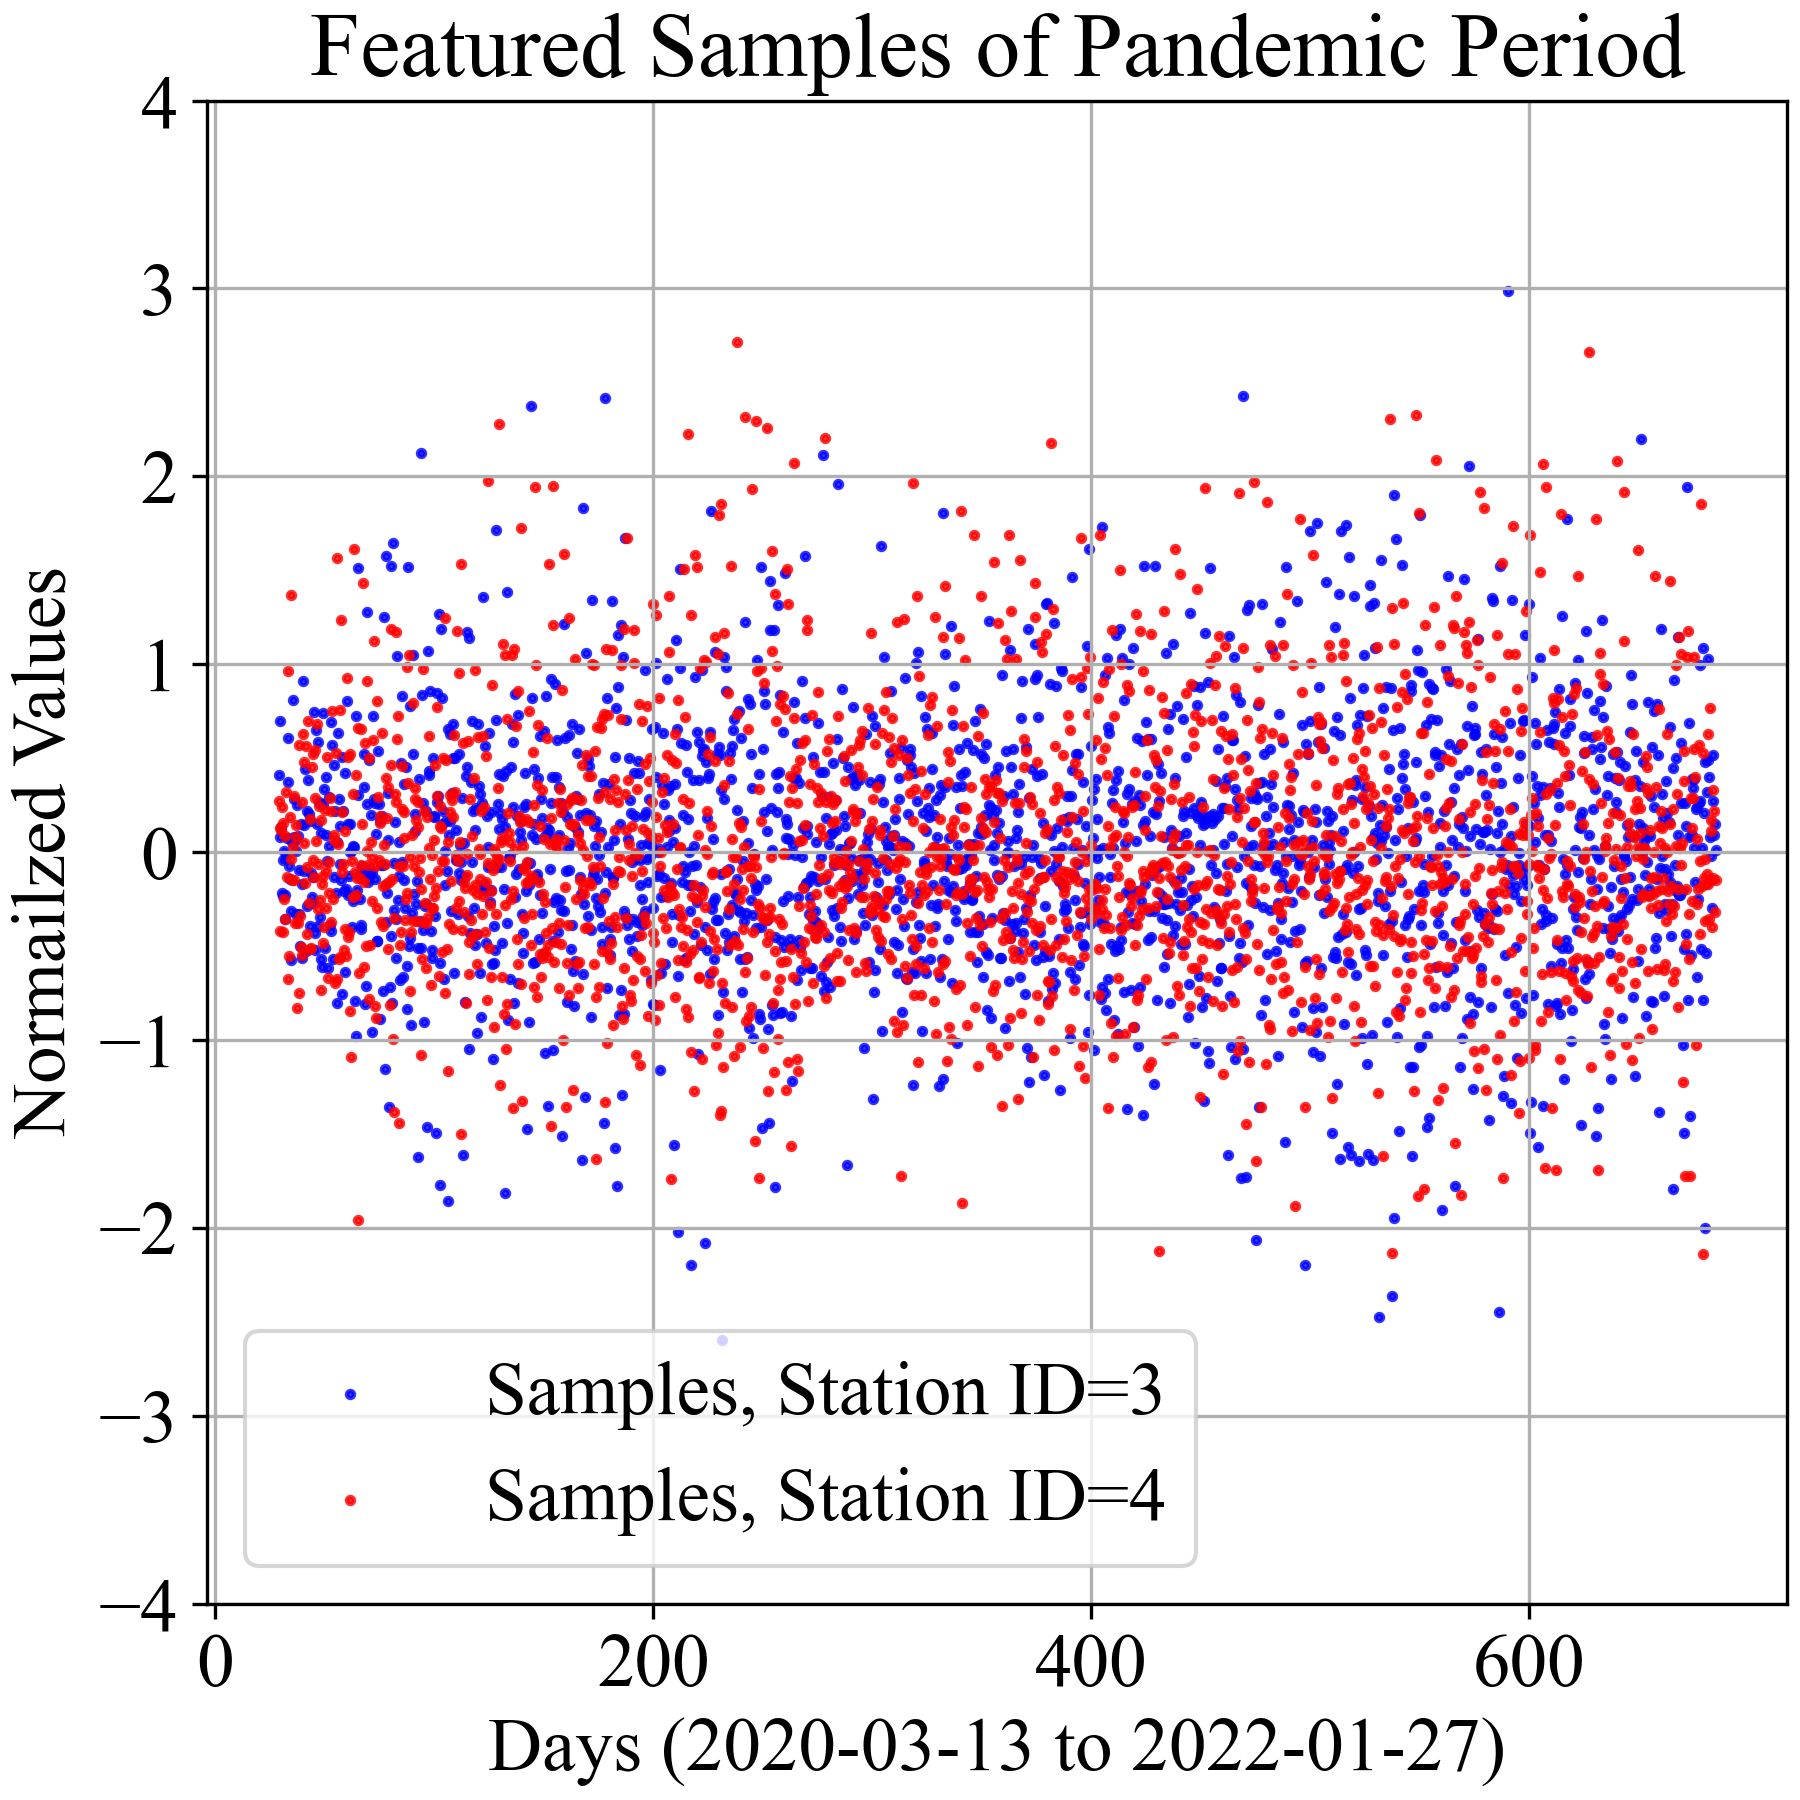
\includegraphics[width=0.35\textwidth]{chap/fig-1.png}
    \caption{
        \footnotesize
        Satellite coordinates of bike stations
        } % 表格标题
    \label{FIGURES: FEATURED DATA}
\end{figure}
% \end{multicols}
% \begin{multicols}{2}
\chapter{M\normalsize{ETHODOLOGY}}
\section{Data Preprocessing}
The strategy had discussed in section \ref{sec:FeatureEngineerforTimeSeries}
demonstrate a method for create new dataset allows model learn 
various cycility in time series. However, for the given dataset which included 
a series of time series for each station respectively. It means that the 
series should be processed specifically for each station. 
\section{Regression Models}
With regression models discussed in lectures, Ridge and Lasso models with 
polynomial features will be evaluated for these tasks. 
Generally for regression model, the algorithm can be abstracted as 
prediction model $f$ and loss function $J$ which 
follow equations \ref{AL}
\end{multicols}
\begin{align}\label{AL}
    \begin{cases}
        \dis 
        \widehat{y} 
        = 
        f(X) = 
        C_{\text{bias}}
        + 
        \sum_{k=0}^{m} 
        \sum_{s=0}^{p}
        \left[
            \sum_{\sum_{i=1}^{k} p_i = s }
            \left(
                \prod_{j=1}^{k}
                \theta_{s}^{kj}x_j^{p_j} 
            \right)
        \right] \: \hspace*{2em} \text{Prediction Model},
        \vspace*{1em}\\
        \dis 
        J(\theta) 
        = 
        \frac{1}{N}
        \sum_{k=1}^{N}
        \left(
            y_{i} - \widehat{y_{i}}
        \right)^2
        + 
        \begin{cases}
            \dis % \alpha
            \frac{||\theta||^2_2}{2C} \: \hspace*{2em} \text{Ridge Model,} 
            \vspace*{1em} \\
            \dis % \alpha
            \frac{||\theta||_1}{2C} \: \hspace*{2em} \text{Lasso Model,}
        \end{cases}
        \: \hspace*{2em} \text{Lost Functions},
    \end{cases}
\end{align}
\vspace*{0.1em}
\begin{multicols}{2}
where $X$ is the dataset with $m$ features, sample size $N$ and polynomial 
featured to $p$ polynomial degree, 
and $C$ and $\theta$ are the trainable parameters for bias term and 
coefficient.
The function $||\cdot||_{n}$ means $n$-norm.
Besides that, loss functions include $L1$ and $L2$ regularization terms with 
$C$ as coefficient penalty for control the sensitivity of model to 
training data which is designed for preventing over-fitting. 
Totally for regression models, the penalty value $C$ and polynomial features $p$ 
are hyperparameters.

% \subsection{Cross Validations}
% In general, $k$-fold cross validation is an approach for tuning models to select 
% hyperparameters from given value lists. 
% However, cross validation is a high computational expensive approach for 
% tuning hyperparameters. 
% Without fine tuning to the hyperparameters of feature engineering to 
% dataset ($q$, $n$, $d$s),
% but exclusively for regression models, hyperparameters are $C$ and $p$ which 
% will be discussed in following sections. 
% \paragraph{Strategy}
% As mentioned, validating in a wide range of values could be computational 
% expensive. 
% Thus, the models Lasso and Ridge will be validated on 
% $C = \left[ 10^{-4}, 10^{-3}, 10^{-2}, 1, 10 \right]$
% and $p = \left[ 1, 2\right]$.
% Furthermore, the full data set of trainable data could be still large to 
% apply validations at this circumstance where 
% totally $5\times 2\times 5=50$ models will be evaluated.
% In order to solving this, the strategy is compromising between 
% the precisions of validations 
% and the computation demands. 
% More specifically, in cross validation process, the training data are only 
% a part of pre-pandemic period which is from 2018-08-01 to 2020-10-31. 
% The details of training is using Adam optimizer at learning rate $10^{-3}$, and 
% $10$ epochs.

% \paragraph{Recommendation of $C$, $p$}
% The results are shown in the figure \ref{FIGURES: Lasso, Ridge, Cross Validation}
% and table \ref{TABLE: MSE of Ridge and Lasso Regression Models on 5-fold cross validation }
% \begin{figure}[htbp]
%     \centering
%     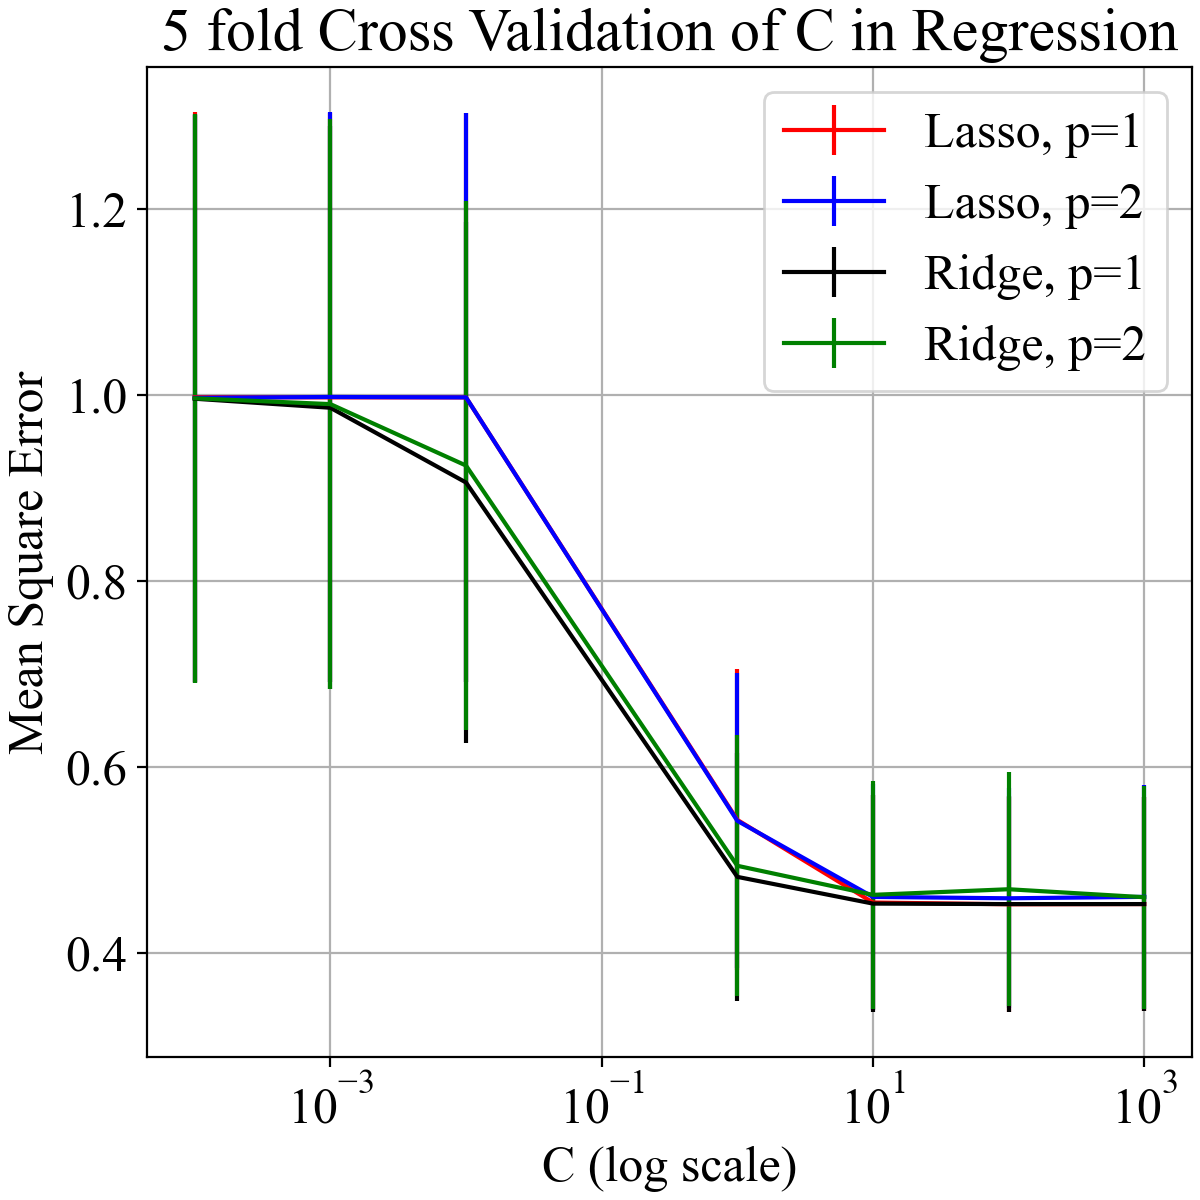
\includegraphics[width=0.4\textwidth]{chap/fig1.png}
%     \caption{
%         \small 
%         MSE of Regression Models $(p=1)$ in
%         $5$-fold cross validation
%         } % 表格标题
%     \label{FIGURES: Lasso, Ridge, Cross Validation}
% \end{figure}
% From the results of $5$-fold cross validation for $C$ and $p$ on Ridge and Lasso regression 
% models shown in figure 
% \ref{FIGURES: Lasso, Ridge, Cross Validation}. 
% It is clear that Lasso and Ridge models have approximately identical 
% performance with non-polynomial featured $(p=1)$ data when penalty 
% value $C = 1$, $10$ and $0.01$.  
% Thus the recommendation of hyperparameter $p$ is $1$. 
% However, as the table shows the mean square error (MSE) of Ridge regression model $(p=1)$
% with $C = 0.01$, it has better performance in validation comparing to 
% Lasso model.
% \begin{table}
%     \small
%     \centering
%         \caption{
%         \small 
%         MSE of Regression Models $(p=1)$ in
%         $5$-fold cross validation
%         } % 表格标题

%     \begin{tabular}{ccccc} % 5列,全部居中对齐
%         \toprule % 顶线
%         $C$ & $0.001$ & $0.01$ & $0.1$ & $1$ \\ % 表头
%         \midrule % 中线
%         Ridge & 160.37 & 88.203 & 81.592 & 81.583 \\ % 第一行数据
%         Lasso & 96.462 & 82.462 & 81.567 & 81.448 \\ % 第二行数据
%         \bottomrule % 底线
%     \end{tabular}
%     \label{TABLE: 
%         MSE of Ridge and Lasso 
%         Regression Models on 
%         5-fold cross validation    
%     } % 用于引用表格的标签
% \end{table}

% \subsection{Predictions}

\section{Long-Short Term Memory (LSTM)}
Traditionally, the Neural Networks or usually called 
Native Neural Networks receive one array as input and 
generate an array as output.
However, there are many tasks required to receive more than one arrays 
as input and produce a sequence of information as output. 
Commonly, the time series prediction tasks and the translation tasks 
required input a sequence of words and output 
a sequence of words as well while the
Recurrent Neural Networks (RNN) allow the model to handle these tasks.
\subsection{Architecture}
The given time series data with different time stamps are denoted with 
a sequence $\{x_t\}_{t=1}^{N}$.
\paragraph{Native RNNs}
Native RNNs at each time step take an input frame $(x_i)$ and 
a history from previous time step $h_{i-1}$ as inputs to 
generate an output $y_i$ and update its history $h_i$. 
Precisely, the RNNs can be represented as a iteration formula of 
kernel function $f_W$ with wights $W$: 
\begin{equation}\label{EQ: 2.1}
    h_i = f_W(h_{i-1}, x_i), \: i = 1, 2, \cdots, t    
\end{equation}
and for common cases, the function $f_W$ is a activation function 
applied to a multiplication of blocked matrixes 
$W = [W_{hh}, W_{xh}]$ and $[h_{i-1}, i_t]$. 
The activation function has various choices: 
$\tanh$, $\text{ReLU}$ and Sigmoid $\sigma$ ect. which are discussed
in lectures. 
Conventionally choose $\tanh$ as activation function for history at time 
stamp $i$, 
\[
    h_i = 
    \tanh
    \left(
        \begin{bmatrix}
            W_{hh} & W_{hx} \\
        \end{bmatrix}
        \begin{bmatrix}
            h_{i-1} \\ x_i \\
        \end{bmatrix}
    \right) + W_{\text{bias}}
\]
Native RNNs have vanishing gradient problem, since the model 
update the wights $W_{hh}$ by getting the derivative of loss at 
every last time stamp $J_i$.
The partial derivative follows 

\begin{align*}
    \frac{
        \partial
        J_i
        }{W_{hh}}
    & =
    \frac{
        \partial J_i
    }{\partial h_i}
    \frac{
        \partial h_{i}
    }{\partial h_{i-1}}
    \cdots
    \frac{
        \partial h_1
    }{\partial W_{hh}}\\
    &
    = 
    \frac{
        \dis 
        W_{hh}^{t-1} 
        \frac{
            \partial J_i
        }{\partial h_i}
        \frac{
            \partial h_1
        }{\partial W_{hh}}
    }{
        \dis 
        \prod_{i=2}^{t}
        \left[1
        +
        \left(\begin{bmatrix}
            W_{hh} & W_{hx} \\
        \end{bmatrix}
        \begin{bmatrix}
            h_{i-1} \\ x_i \\
        \end{bmatrix}
        \right)^2
        \right]}
\end{align*}
Since the part of denominator is always a product of 
a sequence of number larger than $1$, the gradient 
will converge to $0$ as the total time stamps $t$ goes larger.
Considering this case, instead using Native RNNs to these tasks, the optimized RNNs those 
are called Long-Short Term Memory (LSTM) RNNs. 

\paragraph{Long-Short Term Memory} 
LSTM \cite{article} is a type of RNN, which was first announced in 1997 
by Sepp Hochreiter and Jürgen Schmidhuber,
solved vanishing gradient problem. 
At every $t$ time stamp of LSTM model, it has history state $h_{t-1}$ and 
an additional cell state $C_{t-1}$, using both of them and $x_t$ to 
generate history and cell in next state. 
More precisely, the cell and history state stand for different role.
The additional cell state stands for holding the long-term information while the 
history state holds the short-term information controversially. 
The $i$, $f$ and $o$ with independent weights,
correspond the "input", "forget" and "output" 
gates which values are embraced in the interval $[0,1]$ by sigmoid $\sigma$ function. 

\begin{figure}[H]
    \centering
    \begin{tikzpicture}[
        % Define styles
        gate/.style={rectangle, draw, fill=orange!30, minimum size=10mm},
        operator/.style={circle, draw, fill=blue!30, minimum size=10mm},
        function/.style={ellipse, draw, fill=green!30, minimum size=10mm},
        pathline/.style={-latex'},
        scale=0.7, transform shape, every node/.style={scale=0.8, font=\Large}
    ]

        % Nodes
        \node [gate] (forget) {$f$};
        \node [gate, right=of forget] (input) {$i$};
        \node [gate, right=of input] (cell) {$g$};
        \node [gate, right=of cell] (output) {$o$};
        
        \node [operator, right=1cm of output] (times1) {$\odot$};
        \node [operator, above=1cm of times1] (tanh) {tanh};

        \node [operator, above=1cm of input] (times2) {$\odot$};
        \node [operator, above=0.9cm of times2] (plus) {$+$};

        \node [operator, above=2.7cm of forget] (times3) {$\odot$};

        \node [right=8cm of times3] (ct) {$C_t$};
        \node [below=5cm of ct] (ht) {$h_t$};
        \node [above=0.05cm of ht, xshift=-0.4cm] (word1) {or prediction};
        \node [above=0.05cm of word1] (word2) {Higher layer};

        \node [left=1.22of times3] (c-1) {$C_{t-1}$};
        \node [below=5cm of c-1] (h-1) {$h_{t-1}$};

        % Connectors
        \draw [pathline] (times3) -- (plus);
        \draw [pathline] (plus) -- (ct);
        \draw [pathline] (c-1) -- (times3);

        \draw [pathline] (plus) -| (tanh);
        \draw [pathline] (tanh) -- (times1);
        \draw [pathline] (output) -- (times1);

        % \draw [pathline] (times1) -- (plus);
        \draw [pathline] (forget) -- (times3);
        \draw [pathline] (input) -- (times2);
        \draw [pathline] (cell) |- (times2);
        \draw [pathline] (times2) -- (plus);

        \draw [pathline] (h-1) -- (ht);
        \draw [pathline] (times1) |- (ht);

    \end{tikzpicture}
    \caption{
        \footnotesize 
        Workflow of single LSTM unit in LSTM RNN model
        }
    \label{fig: LSTM high way}
\end{figure}
Overall, the formulas of gates operated 
as the equation \ref{EQ: 2.1} and the workflow of LSTM to update 
history and cell states are 

\[
    c_t = f_t\odot c_{t-1} + i_t \odot g_t
\]
\[
    h_t = o_t \odot \tanh(c_t)
\]
The figure \ref{fig: LSTM high way} shows the workflow of LSTM model. 
where the $\odot$ is an element-wise Hadamard product.
The state $h_t$ means the history state which is the state of higher 
layer in model or the prediction of the model. 
Totally, for a $n$ units LSTM model, it has parameters 
$4n(n_{\text{feature}} + n + 1)$ while the number of units is 
hyperparameter of LSTM model.

\paragraph{LSTM RNN for these tasks}
For these tasks, using the simplest LSTM model with single LSTM layer with 
$n$ units and one fully connected layer for prediction. 
Thus, the only hyperparameter is number $n$ of units which needed to 
fine tuning. 

% \end{multicols}
% \begin{multicols}{2}

\section{Evaluation}

\subsection{Cross Validations}\label{SECTION: CROSS_VALIDATION}
The hardware used in following sections is Intel i5-12450H CPU 
with 16 GB DDR5 2133MHz memory and 
NVDIA GeForce 4050 GPU with 6GB GDDR5 memory.

In general, $k$-fold cross validation is an approach for tuning models to select 
hyperparameters from given value lists. 
However, cross validation is a high computational expensive approach for 
tuning hyperparameters. 
Without fine tuning to the hyperparameters of feature engineering to 
dataset ($q$ step ahead, $n$ stamps prediction, $d$ sample cycility),
but exclusively for regression models, hyperparameters are $C$, $p$ 
and for LSTM models number of units 
which will be discussed later. 
\paragraph{Strategy}
As mentioned, validating in a wide range of values could be computational 
expensive. 
Thus, the models Lasso and Ridge will be validated on 
$C = \left[ 10^{-3}, 10^{-2}, 1, 10,100,1000 \right]$
and $p = \left[ 1, 2\right]$. 
The LSTM Models will be evaluated with 
number of units in candidates $[1, 50, 100, 1000]$. 
Furthermore, the full data set of trainable data could be still large to 
apply validations at this circumstance where 
totally $5\times 2\times 6=60$ regression models will be evaluated at least.
In order to solving this, the strategy is compromising between 
the precisions of validations 
and the computation demands. 
More specifically, in cross validation process, the training data are only 
a part of pre-pandemic period which is from 2018-08-01 to 2020-10-31. 
The details of training is using Adam optimizer at learning rate $10^{-3}$, and 
$10$ epochs, and the batch size is $32$.
\subsection{Recommendations}
\paragraph{Recommendation of $C$, $p$}

The results are shown in the \ref{FIGURES: Lasso, Ridge, Cross Validation}
and \ref{TABLE: MSE of Ridge and Lasso Regression Models on 5-fold cross validation }
From the results of $5$-fold cross validation for $C$ and $p$ on Ridge and Lasso regression 
models shown in  
\ref{FIGURES: Lasso, Ridge, Cross Validation}. 
It is clear that Lasso and Ridge models have approximately identical 
performance with non-polynomial featured $(p=1)$ data when penalty 
value $C = 1$, $10$, $0.01$ and up to $1000$.  
Thus the recommendation of hyperparameter $p$ is $1$
for computation resources saving. 
\begin{figure}[H]
    \centering
    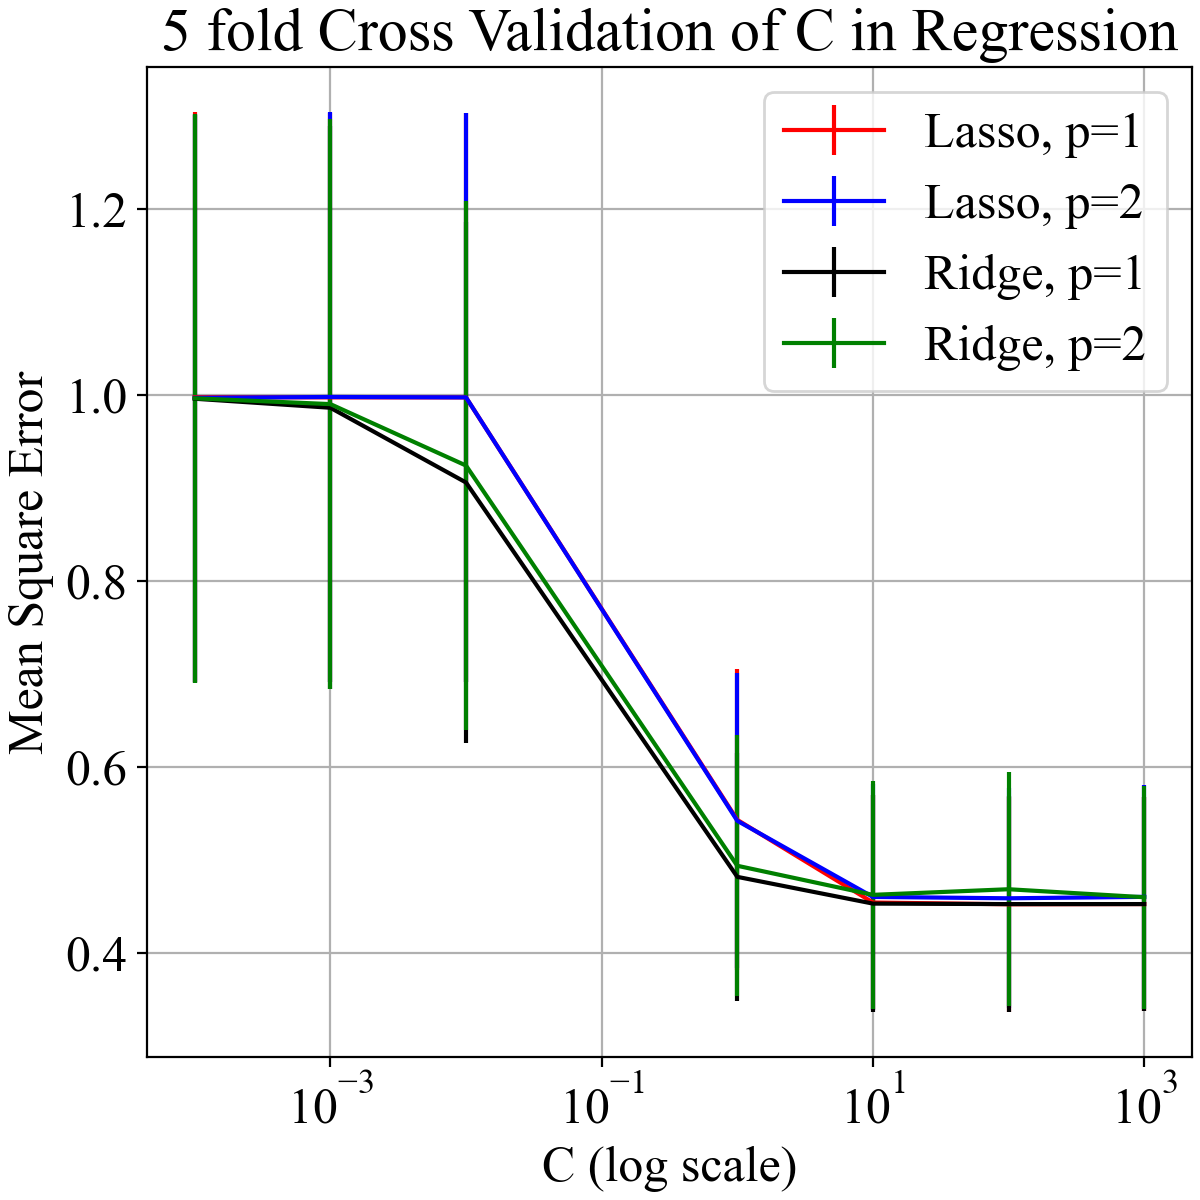
\includegraphics[width=0.4\textwidth]{chap/fig1.png}
    \caption{
        \footnotesize
        MSE of Regression Models $(p=1)$ in
        $5$-fold cross validation
        } % 表格标题
    \label{FIGURES: Lasso, Ridge, Cross Validation}
\end{figure}
However, as the \ref{TABLE: MSE of Ridge and Lasso Regression Models on 5-fold cross validation } shows the mean square error (MSE) of Ridge regression models $(p=1)$
with such various penalty values have same performance as Lasso models. 
Overall, the information of $5$-fold cross validation on Lasso and Ridge models 
does not capable to give a convinced recommendation of hyperparameter $C$.
\begin{table}[H]
    \footnotesize
    \centering
        \caption{
            \footnotesize
        MSE of Regression Models $(p=1)$ in
        $5$-fold cross validation
        } % 表格标题
    \begin{tabular}{ccccc} % 5列,全部居中对齐
        \toprule % 顶线
        $C$ & $1$ & $10$ & $100$ & $1000$ \\ % 表头
        \midrule % 中线
        Ridge & 0.48195 & 0.45320 & 0.45266 & 0.45269 \\ % 第一行数据
        Lasso & 0.54323 & 0.45435 & 0.45247 & 0.45269 \\ % 第二行数据
        \bottomrule % 底线
    \end{tabular}
    \label{TABLE: 
        MSE of Ridge and Lasso 
        Regression Models on 
        5-fold cross validation    
    } % 用于引用表格的标签
\end{table}

\paragraph{Recommendation of units number}
In the case that regression models have approximately identical performance,
the additional LSTM models with $[1, 50, 100, 1000]$ units will be evaluated 
using the strategy in section \ref{SECTION: CROSS_VALIDATION}.
The results of MSE are shown in the \ref{FIGURES: LSTM, Ridge, Cross Validation},
as well as the recommended Ridge Model with 1-polynomial featured data.

With results from the regression models (treated as baseline models),
in the \ref{FIGURES: LSTM, Ridge, Cross Validation}, 
it is clear that LSTM models have better performance comparing 
to the fine tuned Ridge and Lasso models at the beginning ($1$ unit).
\begin{figure}[H]
    \centering
    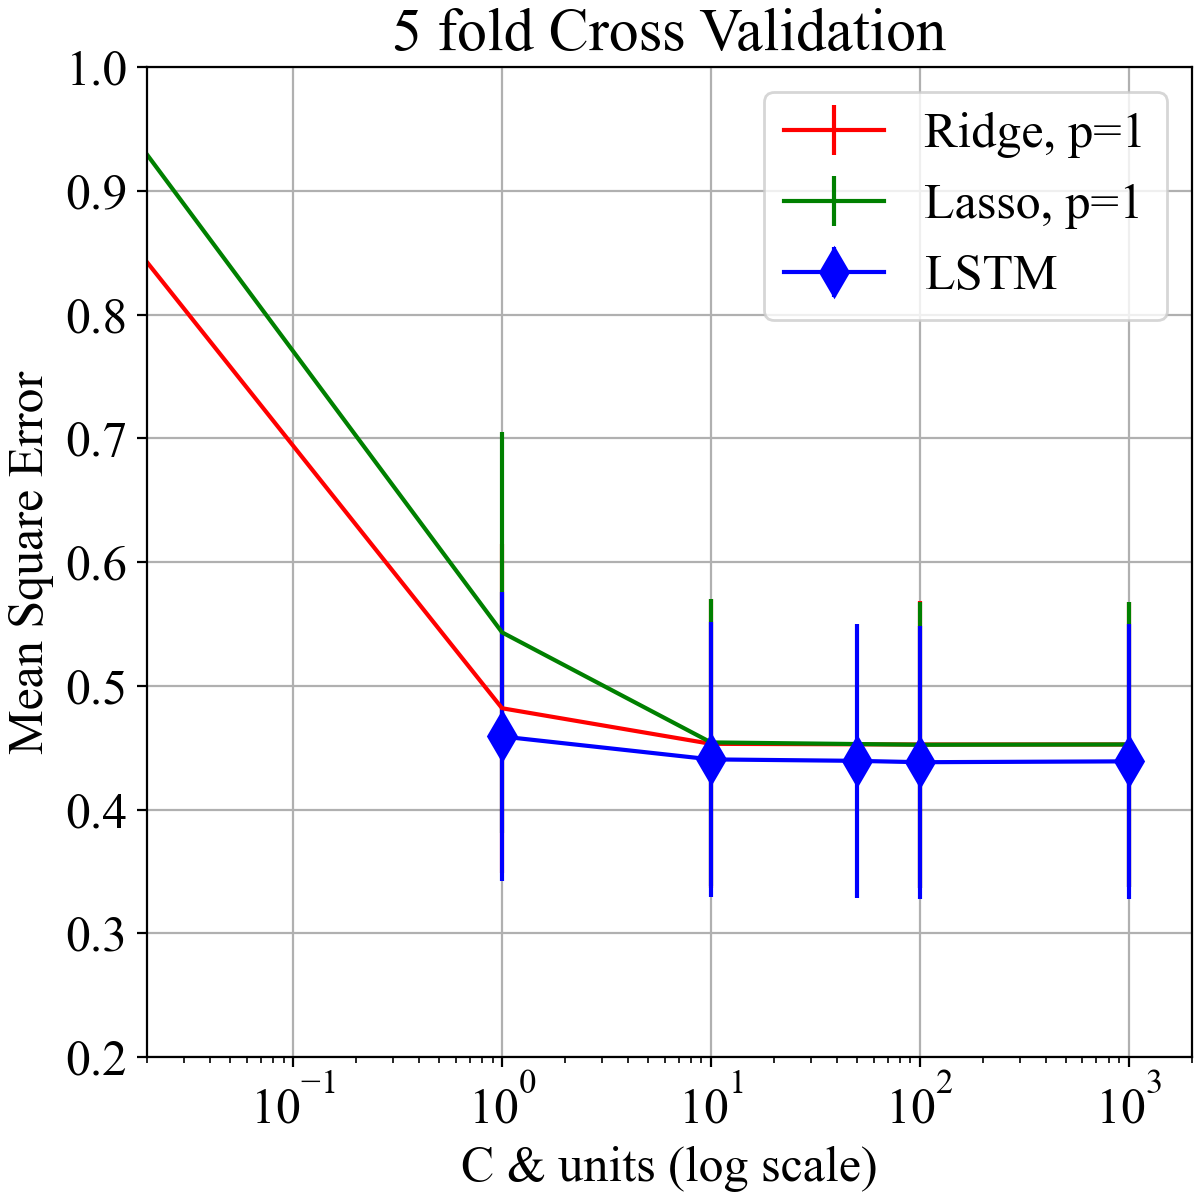
\includegraphics[width=0.4\textwidth]{chap/fig2.png}
    \caption{
        \footnotesize 
        MSE of Regression Models $(p=1)$ in
        $5$-fold cross validation
        } % 表格标题
    \label{FIGURES: LSTM, Ridge, Cross Validation}
\end{figure}
The performance of LSTM model gets to bottleneck as it has around 1000 units 
(due to the limits of hardware, the LSTM which has more units are not capable 
to evaluate). 
\begin{table}[H]
    \footnotesize
    \centering
        \caption{
            \footnotesize
            LSTM RNN model $5$-fold cross validation
        } % 表格标题
    \begin{tabular}{ccccc} % 5列,全部居中对齐
        \toprule % 顶线
        units & $1$ & $10$ & $100$ & $1000$ \\ % 表头
        \midrule % 中线
        LSTM & 0.48195 & 0.45320 & 0.45266 & 0.45269 \\ % 第一行数据
        \bottomrule % 底线
    \end{tabular}
    \label{TABLE: LSTM CROSS VALIDATION   
    } % 用于引用表格的标签
\end{table}
Comparatively, choosing 100 as the number of units is a balance between 
computational cost and performance gained. 

\section{Training LSTM Model}
Considering the recommendations of hyperparameter and 
comparison between regression models and LSTM RNN, the LSTM RNN model 
with a 100 units LSTM layer and a dense layer makes the predictions.
\subsection{Training Settings}
In this case, use the LSTM model with same architecture applied in 
cross validations which is one LSTM layer and one dense layer (prediction layer).
Choosing the training epoch as maximum 100 epoch to ensure the model
sufficiently learned the trends in the given data (pre-pandemic period).
Besides that, in oder to prevent over-fitting, the training strategy includes 
early stopping which means the training process will stop as the metrics of 
fitting process satisfies criterion of tolerance. 

The optimizer of fitting is Adam optimizer same as which applied in validation, 
using the default learning rate setting $(10^{-3})$. 
The batch size is $32$ and 
the tolerance of early stopping is $10^{-4}$,
the patience is $10$ epochs, and it is monitored by validation mean square error 
(mse). 
\begin{figure}[H]
    \centering
    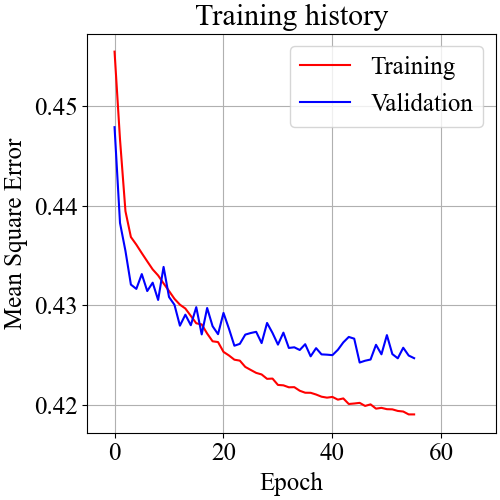
\includegraphics[width=0.35\textwidth]{chap/fig3.png}
    \caption{
        \footnotesize
        Training history of LSTM RNN model on pre-pandemic dataset with 
        100 epochs(stopped at 63th), 32 batch size and Adam optimizer.}
    \label{FIG: Training history of LSTM RNN model on pre-pandemic dataset with 
    50 epochs, 32 batch size and Adam optimizer.}
\end{figure}
\subsection{Results \& Discussion}
The training process early stopped at $56$th epoch iteration where the training 
mse minimized to $0.4202$ and the validation mse is $0.4263$. 
The figure 
\ref{FIG: Training history of LSTM RNN model on 
pre-pandemic dataset with 50 epochs, 32 batch size and Adam optimizer.}
demonstrates that the validation mse did not increase but 
entered the plateau around $40$.
In addition, the mse on testing dataset are $0.4396$ which is close to the validation 
mse. It means that the model learned the general trends behind the given data files.
Therefore, the prediction of the this model could be relatively trustable.
% \begin{multicols}{2}
\chapter{Evaluation}
In this part, using the trained LSTM RNN model in last section to make 
predictions on pandemic and post-pandemic date sets. 
Evaluate the results of the predictions and 
assess the impact of the pandemic on Dublin city-bike usage.
\section{Predictions}
Using the trained model to make predictions on pandemic period and 
post pandemic bike-usage data. 
Comparing the predictions with the collected data to assess the impact of 
pandemic.
Without considering the usage specifically for each station, 
generally predict the full dataset is the simple way to assess the differences.
The \ref{FIGURES: Predictions Samples of Pandemic Period}
shows a brief view of predictions and sample values.
Although there are differences can be determine from the figures 
(post-pandemic period \ref{FIGURES: Predictions Samples of POST Pandemic Period}
and pandemic period \ref{FIGURES: Predictions Samples of Pandemic Period}), 
the qualitative analysis should be applied.

\paragraph{Qualitative Analysis}
In order to determine the differences between theoretical prediction and the 
real values, there are many methods to do so. 
\begin{figure}[H]
    \centering
    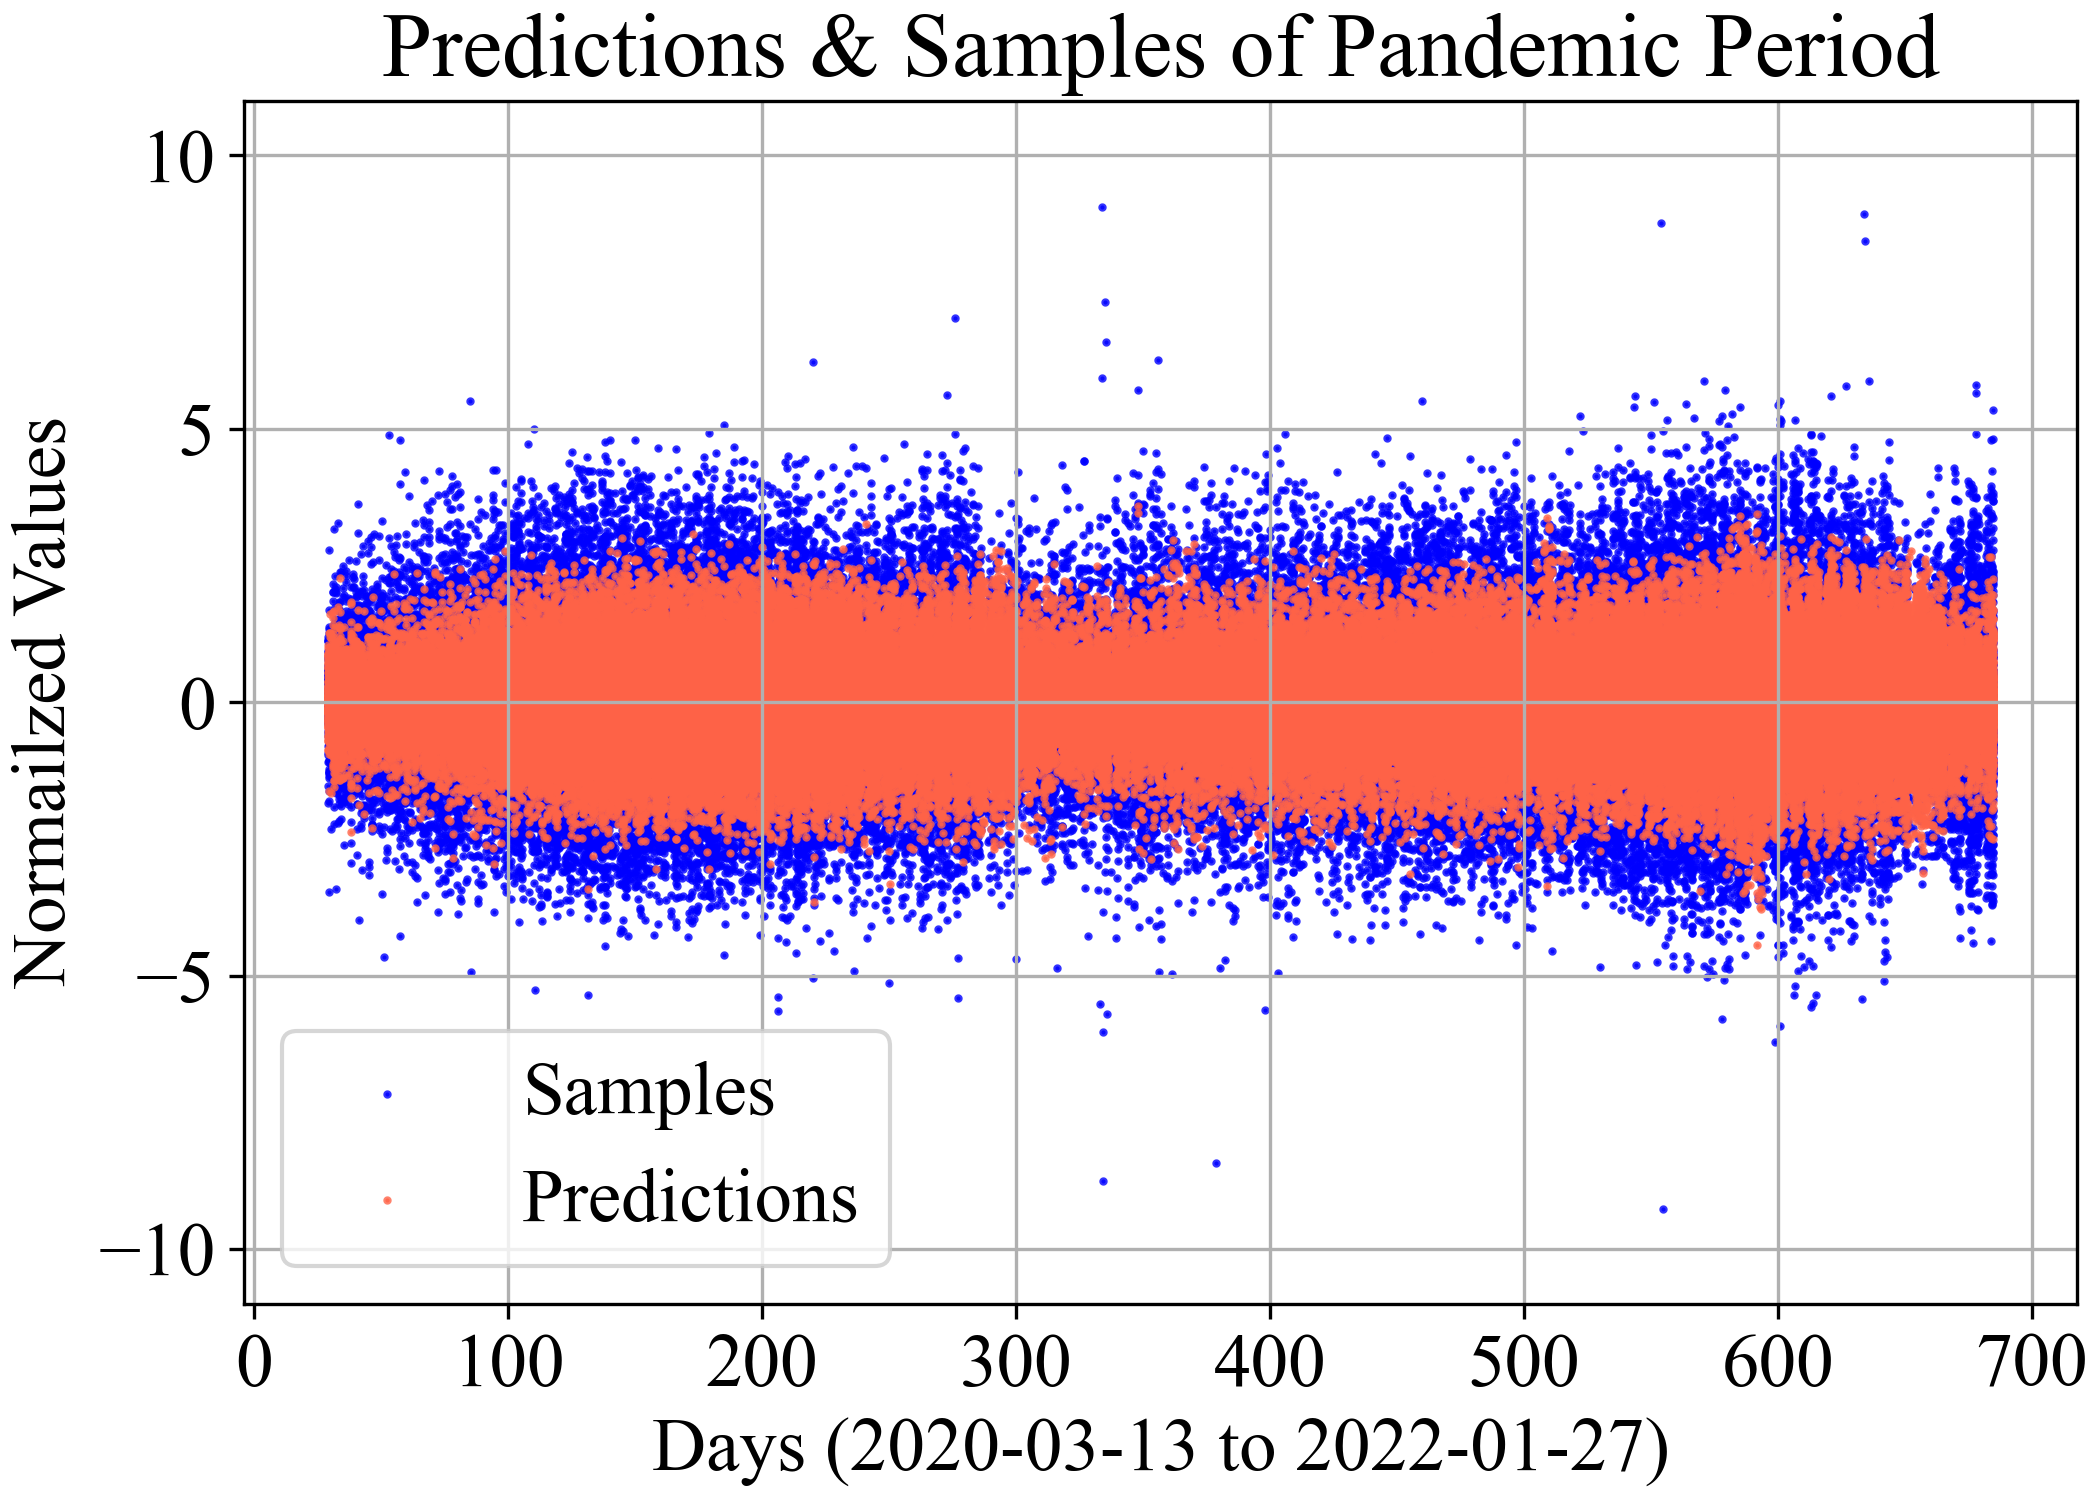
\includegraphics[width=0.45\textwidth]{chap/fig5.png}
    \caption{
        \footnotesize 
            Predictions \& Samples of Pandemic Period
        } % 表格标题
    \label{FIGURES: Predictions Samples of Pandemic Period}
\end{figure}
But for simply purpose rather than the most precisely purpose, 
using the 'Bootstrap' to analysis the results since it is an 
efficient method to evaluate the performance and the reliance of model.

In this case specifically, randomly select a part of ($20\%$) the given dataset,
and evaluate the performance of the model on this fraction of sample. 
Totally, this process is looped $1000$ iterations. 
In more complex cases, the size of selected data samples and the number of iterations
are also required to determine by fine-tuning methods, since they are hyperparameter
as well. 
The 
\begin{figure}[H]
    \centering
    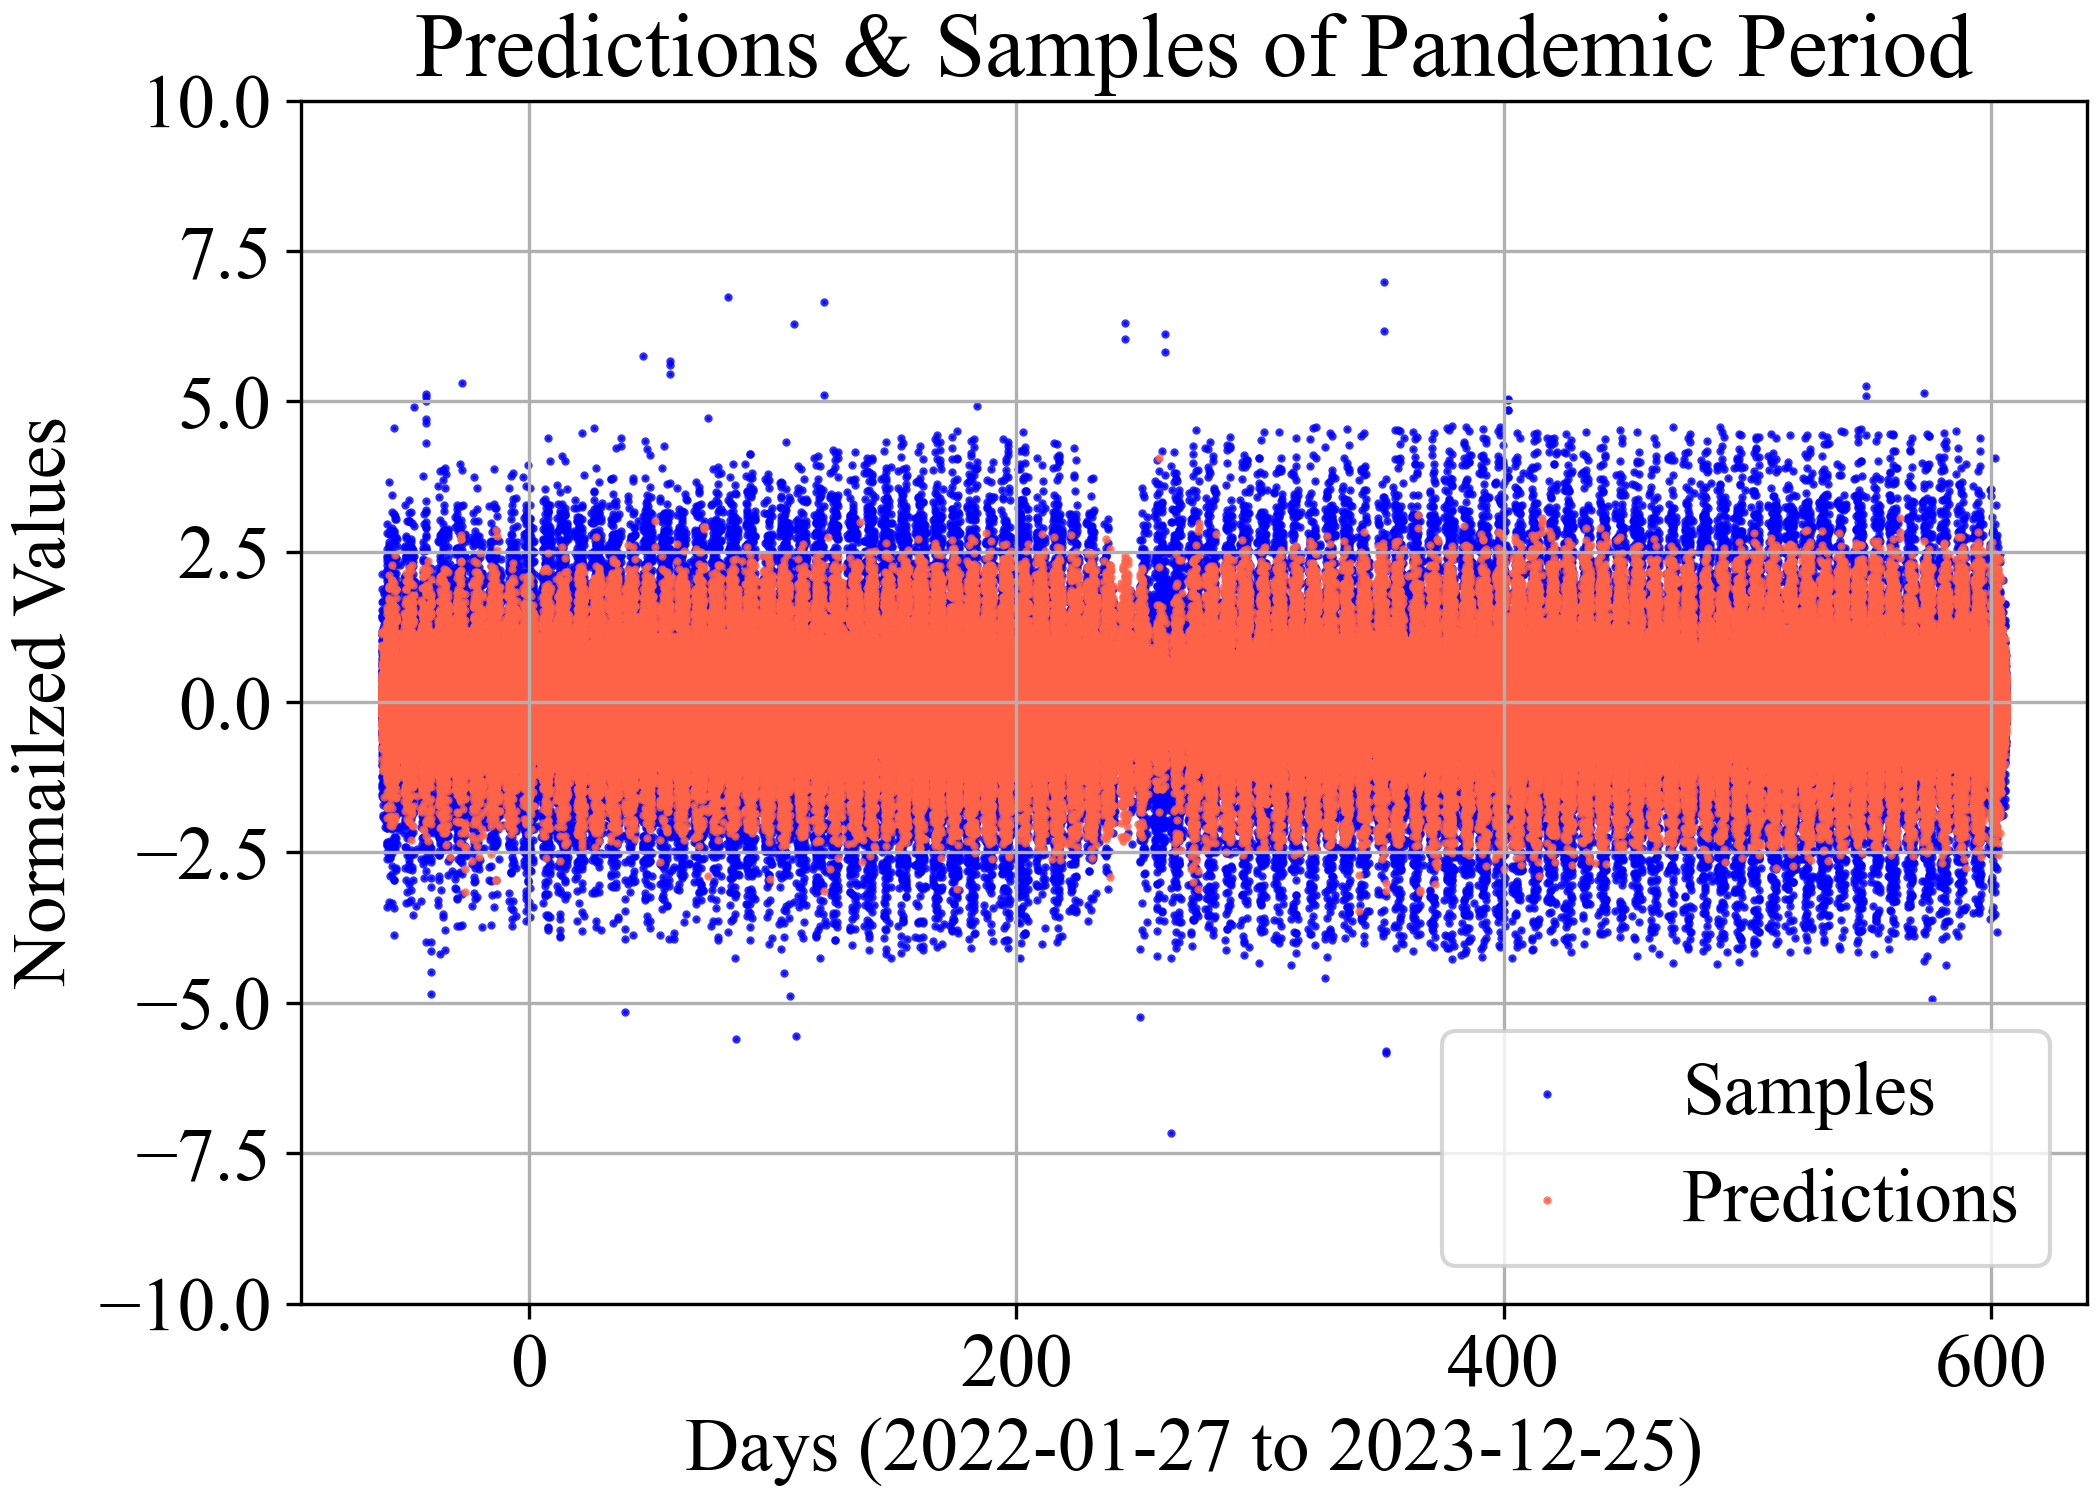
\includegraphics[width=0.45\textwidth]{chap/fig6.png}
    \caption{
        \footnotesize 
            Predictions \& Samples of Post-Pandemic Period
        } % 表格标题
    \label{FIGURES: Predictions Samples of POST Pandemic Period}
\end{figure}
The results of Bootstrap are shown in the table below \ref{TABLE: BOOTSTRAP DUR POST PRE } 
\begin{table}[H]
    \footnotesize
    \centering
        \caption{
            \footnotesize
            Mean \& standard deviation of Bootstrap results
        } % 表格标题
    \begin{tabular}{cccc} % 5列,全部居中对齐
        \toprule % 顶线
        periods & pre-pandemic & pandemic & post-pandemic \\ % 表头
        \midrule % 中线
        mean & 0.42277 & 0.8149587 & 0.478253  \\ % 第一行数据
        std & 0.00581216 & 0.0106626 & 0.005191669 \\ % 第一行数据
        \bottomrule % 底线
    \end{tabular}
    \label{TABLE: BOOTSTRAP DUR POST PRE
    } % 用于引用表格的标签
\end{table}
\paragraph{Discussion of pandemic period}
In \ref{TABLE: BOOTSTRAP DUR POST PRE }, it is clear to determine 
that the mean value of scores of Bootstrap (mse) in pandemic period
are much more higher than pre and post pandemic period, the 
standard deviation as well. 
It means that the impact of the pandemic to the bike-usage are 
significantly large compare to before and after it happened.
Also, it shows that the bike-usage in pandemic period 
are more unstable.

\paragraph{Discussion of post-pandemic period}
In \ref{TABLE: BOOTSTRAP DUR POST PRE }, comparing to the pre-pandemic and 
pandemic period, the bike-usage is slightly larger than pre-pandemic but 
much more smaller than pandemic period. 
It means that the bike-usage was sufficiently recovered after city lock-down ended.
And the bike-usage approximately recovered to the level as pre-pandemic period.
Besides that, the trend of bike-usage recovery is stable through 
observing the deviation which is approximately same but still smaller than pre-pandemic 
period. 

    
\chapter{Q\normalsize{UESTIONS}}
\titleformat{\paragraph}[runin]
{\normalsize\itshape\bfseries}{\theparagraph}{1em}{}

\thequestion What is a ROC curve? How can it be used to evaluate the performance of a classifier
compared with a baseline classifier? Why would you use an ROC curve instead of a
classification accuracy metric? 
\refstepcounter{question}

\paragraph{Answer}
For the two-feature classification task
which the data are labeled only two type of classes. 
Conventional choice is linear model $y = \theta^{\text{T}} X$ 
which is to predict whether label associated with feature vector $X$ is $1$ or $−1$ 
generally, with decision boundary $\alpha$.
Commonly used, is the true-positive (TP), false-positive (FP) rates which mean 
the model predicted the positive label right and false.
As vary the parameter $\alpha$ the balance of true-positive and false-positive rates.
A ROC curve is a plot of true positive rate vs false
positive rate.

\paragraph{Answer}
The accuracy of predictions is $\frac{TP}{FP+TP}$, thus the idea classifier 
has 100\% TP and 0\% FP. 
The idea classifier gives a point $(0,1)$ at the upper-left conner of 
ROC plot. 
The baseline classifier which just predict the most frequent feature or 
just random feature, gives a point on the $y=x$ line.
So the way of ROC evaluate the performance of classifier is to 
determine how close of the ROC curve of the classifier to the upper-left conner of 
the region $[0,1]\times [0,1]$.

\paragraph{Answer}
Using accuracy as metrics have problem when handle imbalanced datasets.
If there are 90\% samples are labels as A 10\% as B, the most frequency 
baseline model will have 90\% accuracy.
However, this doesn't necessarily indicate good performance in recognizing the minority class
which means accuracy is not a good assessment.
ROC curves provide a more comprehensive performance assessment 
by considering both the true positive rate and false positive rate.

The ROC curve provide a full view of performance under various thresholds $\alpha$.
While accuracy is based on a specific decision threshold (just one point), 
which may not always be apparent, 
especially in cases where some classes are more critical than others. 
The ROC curve shows how various thresholds affect the performance of classifier.

Also the ROC curve provide full information to designers which allows to 
choice the threshold $\alpha$ with different tolerance of FT and TP.
Besides that, the ROC curve make it is easier to compare the performance of 
different classifiers by visually approximately determine which classifier 
with which tolerance $\alpha$ is they needed.

\vspace{1em}
\thequestion Give two examples of situations where a linear regression would give inaccurate
predictions. Explain your reasoning and what possible solutions you would adopt in each
situation.
\refstepcounter{question}

\paragraph*{Answer}
There are many cases that linear regression models are more likely to give inaccurate
predictions.
\paragraph{Example}
Linear model assume that the liner relationships among the samples which
are independent and dependent related. 
Such as the samples sets $\{(x_{k}, y_k)\}_{k=1}^{N}$ where 
$X = \{x_k\}_{k=1}^{N}$ and $y_{k} = f(x_k) = x_k^2$ (quadratic related).
The linear model $\widehat{f}(x) = \theta_1 x + \theta_0$ is not able to capture the non-linear relationship in this 
sample sets.
Therefore, it will make inaccurate predictions, although it was trained.
\paragraph{Solution}
In this case, if keeping using linear model, the solution commonly is to 
feature engineering the sample set $\{(x_{k}, y_k)\}_{k=1}^{N}$ with $2$ polynomial features.
The new sample set will be composed by $(x_{k}, x^2_{k}, y_k)$. 
Furthermore, the linear model $\widehat{f}$ is a equation below
\[
    \widehat{y_k} = \widehat{f}(x_{k}, x^2_{k}) 
    = \theta_2 x_k^2 + \theta_1 x_k + \theta_0
\]
At this case, the new linear model trained on featured sample set could learn the quadratic
relationships among the sample set.

\paragraph{Example}
Linear model, also other models, have higher chance to make inaccurate predictions
as long as the samples are not preprocessed well. 
Such as the presence of out-liner, missing some information and unbalanced samples.
Take the presence of out-liner as an example.

Since linear regression models are sensitive to the samples which are 
significantly different with others, 
especially in the independent variables (predictors).
They can have a disproportionately large influence on the line of best fit. 
This can skew the results of the linear model, leading to inaccurate predictions.

\vspace{1em}
\thequestion The term 'kernel' has different meanings in SVM and CNN models. Explain the two
different meanings. Discuss why and when the use of SVM kernels and CNN kernels is
useful, as well as mentioning different types of kernels.
\refstepcounter{question}
\paragraph{Explainations}
In Kernel SVMs, 
a kernel is a \underline{function} $\kappa$
used for transforming the data into a higher dimension 
where a linear separator might be found. 
It can be represented as $\kappa(x_{i}, x_{j}) = \phi(x_i)^{\text{T}}\phi(x_j)$
which is the dot product of data points 
in a transformed feature space 
enabling the SVM to classify data that 
is not linearly separable in the original space.
The primary purpose of using a kernel in SVMs 
is to solve nonlinear relationships 
by applying a linear classification approach. 
Common kernels include linear combination, polynomial, and sigmoid ($\sigma$). 

In CNNs, a kernel (or filter) refers to a small \underline{matrix} used to extract 
features from input data (especially for image classification tasks such as 
ImageNet Challenge) through a process called convolution and collectively as 
convolution layer. 
The kernel slides (shift) over the input data, 
performing element-wise multiplication 
and sum subsequently.
It effectively capturing patterns such as 
edges, shapes, and textures. 
Each kernel in a CNN is trained to identify a specific type 
of feature in the input, and through multiple layers of 
convolutions and other operations, 
CNNs can recognize complex patterns in larger structures such 
as object detection or facial recognition datasets.

\paragraph{Reasons}
In many real-world scenarios, data is not linearly separable. 
Kernel SVMs allow these datasets to be transformed 
into a higher-dimensional space without loosing no-linear relationships,
where a linear separator can be found. 
Moreover, the kernel can be applied in any linear model not just for SVMs.
The model $\widehat{f}$ in previous question is an example.

In real-word tasks, the input sample is commonly too large to evaluate 
in single iteration, such as a 4K (4360*2160 pixels) image captioning tasks.
However, by using a series of various size of kernels 
(for RGB image data, commonly 3*3*3, 5*5*3, 7*7*3 small kernels, 
32*32*3, 64*64*3, 96*96*3 large kernels), training them in the process of 
sliding through data, the computational demands are reduced significantly.
Besides that, with different size of kernels, the kernels can learn 
various patterns inside given data which is more complicated to achieve using 
single matrix multiplication. 
Moreover, kernels with different size can learning different features, such 
as using 32*32*3 kernel to learn the feature both in RGB channels, and 
32*32*1 kernel to lean the feature in one channel. 
By combining various type of kernels, the CNN model can learn 
various features in data effectively.

\vspace{1em}
\thequestion In k-fold cross-validation, a dataset is resampled multiple times. What is the idea behind
this resampling i.e. why does resampling allow us to evaluate the generalization
performance of a machine learning model. Give a small example to illustrate. Discuss
when it is and it is not appropriate to use k-fold cross-validation.

\paragraph{Answer}
In real-world case, the researchers want to maximize the utilization of 
collected data. 
However, splitting the dataset into training dataset and testing dataset,
a large portion of data will not used for training which 
have higher chance to be particularly problematic with small datasets. 
Also called the model has not sufficient generalization performance.
On the contrast, $k$-fold cross validation is an approach that 
ensure all sample are utilized for training, but by separating the dataset into 
$k$ parts. 
Since using more data for training, the model will have better generalization
performance.

Besides that, this approach helps researchers identify the 
data-driven issues like over-fitting and under-fitting, 
since the model trained on more data.
After the model trained on better processed dataset, the model will 
have better performance.

\paragraph{Answer}
$k$-fold cross-validation 
is appropriate for small to medium datasets, model selection, 
hyperparameter tuning, and when a robust estimate of model performance is required. 

$k$-fold cross-validation is not suitable for very large datasets due to 
computation resource demands, extremely imbalanced datasets, 
or data with grouped observations, 
as it may disrupt the inherent structure of the data.

\end{multicols}
{
  \small
\bibliographystyle{plain}
\bibliography{bibfile}
}
\chapter{Appendix}
\section{Code}
\subsection{loaddata.py}\label{Metropolis_Uniform}
\lstset{style=PythonStyle}
\begin{lstlisting}
import numpy as np
import pandas as pd
import os
from tqdm import tqdm
from datetime import datetime

# This the file loading all data and return them in 3 type classes (before during after) of pademic period
def generate_filenames(start_year, end_year, pattern):
    filenames = []
    if pattern == 0:
        # Monthly data filenames
        for year in range(start_year, end_year + 1):
            for month in range(1, 13):
                filename = f"dublinbike-historical-data-{year}-{month:02d}.csv"
                filenames.append(filename)
    elif pattern == 1:
        # Quarterly data filenames
        quarters = [(1, 4), (4, 7), (7, 10), (10, 1)]
        for year in range(start_year, end_year):
            for start_month, end_month in quarters:
                start_date = f"{year}{start_month:02d}01"
                end_year_shift = year if end_month != 1 else year + 1
                end_date = f"{end_year_shift}{end_month:02d}01"
                filename = f"dublinbikes_{start_date}_{end_date}.csv"
                filenames.append(filename)

    return filenames


def read_data():
    start_year = 2018
    end_year = 2023
    df = pd.DataFrame()
    # Choose 0 for monthly data, 1 for quarterly data
    for pattern in range(2):
        file_list = generate_filenames(start_year, end_year, pattern)
        for file in file_list: # Loading data
            file_name = "datafiles/" + file
            if os.path.exists(file_name): 
                print(f"Load file: {file_name}")
                data = pd.read_csv(file_name)

                # Unify the colunm indexes
                data.rename(columns = {"AVAILABLE BIKE STANDS": "AVAILABLE_BIKE_STANDS"}, inplace=True)
                data.rename(columns = {"AVAILABLE BIKES": "AVAILABLE_BIKES"}, inplace=True)
                data.rename(columns = {"BIKE STANDS": "BIKE_STANDS"}, inplace=True)
                
                df = pd.concat([df, data], axis=0, ignore_index=True)
    
    station_info_dict = {}
    for id in df["STATION ID"]:
        if id in station_info_dict:
            continue
        else:
            station_info_dict[id] = {
                "NAME": df[df["STATION ID"] == id]["NAME"].values[0],
                "ADDRESS": df[df["STATION ID"] == id]["ADDRESS"].values[0],
                "LATITUDE": df[df["STATION ID"] == id]["LATITUDE"].values[0],
                "LONGITUDE": df[df["STATION ID"] == id]["LONGITUDE"].values[0]
            }
    station_info_dict = dict(sorted(station_info_dict.items(), key = lambda item: item[0]))
    
    df["TIME"] = pd.to_datetime(df["TIME"])
    # Split March 2020 into pre and post pandemic
    # March 13th, the first day schools were closed 
    # (https://www.irishtimes.com/health/2023/05/05/covid-emergency-is-over-20-key-moments-of-pandemic-that-changed-the-world/)
    timepoint_begin = pd.Timestamp('2020-03-13 00:00:00')
    
    # Split January 2022 into pre and post pandemic
    # Jan 28th 2022, the day the HSE stopped releasing COVID-19 figures 
    # (https://www.irishtimes.com/health/2023/05/05/covid-emergency-is-over-20-key-moments-of-pandemic-that-changed-the-world/)
    timepoint_end = pd.Timestamp('2022-01-27 23:59:59')

    df = df.drop_duplicates()
    df_pre = df[df["TIME"] < timepoint_begin]
    df_dur = df[(df["TIME"] >= timepoint_begin) & (df["TIME"] <= timepoint_end)]
    df_post = df[df["TIME"] > timepoint_end]
    
    return df_pre, df_dur, df_post, station_info_dict

# Round a time string to the nearest 5 minutes in a datetime object
def round_to_5_minutes(time_stamp: pd.Timestamp) -> datetime:
    # Parse the input string into a datetime object
    dt = time_stamp.to_pydatetime()

    # Round down to the nearest 5 minutes
    rounded_dt = datetime(dt.year, dt.month, dt.day, dt.hour, (dt.minute // 5) * 5)

    return rounded_dt

# Round a time string to the nearest 8 hour in a datetime object
def round_to_hour(time_stamp: pd.Timestamp) -> datetime:
    # Parse the input string into a datetime object
    dt = time_stamp.to_pydatetime()

    # Round down to the nearest day
    rounded_dt = datetime(dt.year, dt.month, dt.day, (dt.hour // 8) * 8)

    return rounded_dt
    
# Round a time string to the nearest a day in a datetime object
def round_to_day(time_stamp: pd.Timestamp) -> datetime:
    # Parse the input string into a datetime object
    dt = time_stamp.to_pydatetime()

    # Round down to the nearest day
    rounded_dt = datetime(dt.year, dt.month, dt.day)

    return rounded_dt
    
# Combine time/dates into one value per time
def combine_dates(df: pd.DataFrame, period: str) -> pd.DataFrame:
    # Round times to nearest 5 minutes
    # tqdm.pandas(desc=f"Rounding {period} times to closest 5 minutes.")
    # df['TIME'] = df['TIME'].progress_apply(round_to_5_minutes)

    # Round times to nearest a day
    # tqdm.pandas(desc=f"Rounding {period} times to closest day.")
    # df['TIME'] = df['TIME'].progress_apply(round_to_day)

    # # Round times to nearest an hour
    tqdm.pandas(desc=f"Rounding {period} times to closest hour.")
    df['TIME'] = df['TIME'].progress_apply(round_to_hour)

    # Aggregate times together, with all counts summed
    return df.groupby(df['TIME'], as_index=False).aggregate({'BIKE_STANDS': 'mean', 'AVAILABLE_BIKE_STANDS': 'mean', 'AVAILABLE_BIKES': 'mean'})

# Combine time/dates of each station into one value per time
def combine_dates_station(df: pd.DataFrame, info: dict, period: str) -> pd.DataFrame:
    df_new = pd.DataFrame()
    for station in info:
        temp = combine_dates(df[df["STATION ID"] == station], period)
        temp["STATION_ID"] = station
        df_new = pd.concat([df_new, temp], axis=0, ignore_index=True)
    return df_new


# Clean data, fill zeros to un-occured station
from itertools import product
def clean_data(df:pd.DataFrame, info: dict) -> pd.DataFrame:
    station_ids = list(info.keys()) # 从字典中提取站点ID

    # 步骤 1: 创建完整的时间序列
    min_time = df['TIME'].min()
    max_time = df['TIME'].max()
    all_times = pd.date_range(start=min_time, end=max_time, freq='8H') #D for day, H for hour, T for minute

    # 为每个站点创建完整的时间序列
    full_df = pd.DataFrame(list(product(station_ids, all_times)), columns=['STATION_ID', 'TIME'])

    # 合并数据集
    df = df.set_index(['STATION_ID', 'TIME'])
    full_df = full_df.set_index(['STATION_ID', 'TIME'])
    combined_df = full_df.join(df, how='left')

    # 填充缺失值
    combined_df.fillna(method='ffill', inplace=True)
    combined_df.reset_index(inplace=True)
    return combined_df

import json
def main():
    df_pre, df_dur, df_post, station_info = read_data()
    df_pre, df_dur, df_post = combine_dates_station(df_pre, station_info, "pre-pandemic"), combine_dates_station(df_dur, station_info, "pandemic"), combine_dates_station(df_post, station_info, "post-pandemic")
    
    df_pre, df_dur, df_post = clean_data(df_pre, station_info), clean_data(df_dur, station_info), clean_data(df_post, station_info)  

    # 存储和读取 pandas DataFrame,
    df_pre.to_hdf("pre.h5", key='df', mode='w')
    df_dur.to_hdf("dur.h5", key='df', mode='w')
    df_post.to_hdf("post.h5", key='df', mode='w')

    # 将字典写入 JSON 文件
    with open('station_info.json', 'w') as json_file:
        json.dump(station_info, json_file)

if __name__ == "__main__":
    main()
    

\end{lstlisting}
\subsection{preprocessing.py}\label{Metropolis_Uniform}
\lstset{style=PythonStyle}
\begin{lstlisting}
import numpy as np
import pandas as pd

import json
# 从 JSON 文件读取数据到字典
with open('station_info.json', 'r') as json_file:
    station_info = json.load(json_file)

# Feature engineering
def get_featured_data(df, station_info):
    def get_flow(df):
        features = ['STATION_ID', 'TIME', 'TAKE_BIKES']
        data = pd.DataFrame(index=range(df.shape[0] - 1),columns=features)
    
        for i in range(1, df.shape[0]):
            data.iloc[i-1]['STATION_ID'] = df.iloc[i-1]["STATION_ID"]
            data.iloc[i-1]['TIME'] = df.iloc[i-1]["TIME"]
        
            y1 = df.iloc[i-1]["AVAILABLE_BIKE_STANDS"] - df.iloc[i]["AVAILABLE_BIKE_STANDS"]
            y2 = df.iloc[i-1]["AVAILABLE_BIKES"] - df.iloc[i]["AVAILABLE_BIKES"]
    
            # data.iloc[i-1]['BRING_BIKE_STANDS'] = y1
            # data.iloc[i-1]['TAKE_USING'] = y2 + y1
            
            data.iloc[i-1]['TAKE_BIKES'] = y2 + y2 + y1
        return data

    
    for idx, id in enumerate(station_info):
        if idx == 0:
            y = get_flow(df[df["STATION_ID"] == int(id)])
        else:
            y = pd.concat([y, get_flow(df[df["STATION_ID"] == int(id)])], axis = 0)
    y.index = range(y.shape[0])
    return y


def get_trainable_data(df, isolate_station, period):
    # Get the start-end TimeStamps
    if period == 'pre':
        start = pd.to_datetime("01-08-2018", format='%d-%m-%Y')
        end = pd.to_datetime("13-03-2020", format='%d-%m-%Y')
    elif period == 'dur':
        start = pd.to_datetime("13-03-2020", format='%d-%m-%Y')
        end = pd.to_datetime("27-01-2022", format='%d-%m-%Y')
    elif period == 'post':
        start = pd.to_datetime("27-01-2022", format='%d-%m-%Y')
        end = pd.to_datetime("25-12-2023", format='%d-%m-%Y')
    elif period == 'cross_validation':
        start = pd.to_datetime("01-08-2018", format='%d-%m-%Y')
        end = pd.to_datetime("31-10-2020", format='%d-%m-%Y')

    
    # Get full time index
    t_full = pd.array(pd.DatetimeIndex(df.iloc[:,1]).astype(np.int64)) / 1e9
    t_start = pd.DataFrame([start]).astype(np.int64) / 1e9
    t_end = pd.DataFrame([end]).astype(np.int64) / 1e9
    
    t = np.extract([np.asarray(t_full >= t_start[0][0]) &  np.asarray(t_full <= t_end[0][0])], t_full)
    # t.shape
    
    # Get the STATION_ID 
    id = np.extract([np.asarray((t_full>=t_start[0][0])) & np.asarray((t_full<=t_end[0][0]))], df.iloc[:,0]) 

    
    # Get the sampling time period
    dt = t[id == 2][1] - t[id == 2][0]
    # print("Data sampling interval is %d secs." %dt)

    t = (t - t[0]) / 60 / 60 / 24 # convert timestamp to days
    
    y = np.extract([np.asarray((t_full>=t_start[0][0])) & np.asarray((t_full<=t_end[0][0]))], df.iloc[:,2]).astype(np.float64)
    # y.shape
    y = (y - y.mean())/y.std()
    
    if isolate_station:
        y_2d = []
        t_2d = []
        for i in station_info:
            y_2d.append(y[id == int(i)])
            t_2d.append(t[id == int(i)])
        y_2d = np.array(y_2d)
        t_2d = np.array(t_2d)
        return y_2d, t_2d, id, dt
    else:
        return y, t, id, dt


def main(period, isolate_station):
    # isolate_station = False for 1-dim y, True for 2-dim y
    if period == 'pre':
        df_pre = pd.read_hdf('pre.h5', 'df')
        df = get_featured_data(df_pre, station_info)
    elif period == 'dur':
        df_dur = pd.read_hdf('dur.h5', 'df')
        df = get_featured_data(df_dur, station_info)
    elif period == 'post':
        df_post = pd.read_hdf('post.h5', 'df')
        df = get_featured_data(df_post, station_info)
    elif period == 'cross_validation':
        df_pre = pd.read_hdf('pre.h5', 'df')
        df = get_featured_data(df_pre, station_info)
        
    y, t, id, dt = get_trainable_data(df, isolate_station, period)
    
    return y, t, id, dt, station_info
\end{lstlisting}


\subsection{train\_LSTM.py}
\begin{lstlisting}
import pandas as pd
import numpy as np
import sys, math
import matplotlib.pyplot as plt
import tensorflow as tf
epoch = 10

plt.rc('font', size=18); plt.rcParams['figure.constrained_layout.use'] = True

import preprocessing
isolate_station = False
y, t, id, dt, station_info = preprocessing.main('cross_validation', isolate_station)

#plot extracted data
# plt.scatter(t[id==10], y[id==10], c='b', marker='+',s=2)
# plt.scatter(t[id==4], y[id==4], c='r', marker='+',s=2); plt.show()


def feature_all_time_series(q = 3, lag = 3):
    def feature_time_series(q, lag, plot, y, t, id, dt):
    # q-step ahead prediction
        stride = 1

        # m = math.floor(30*7*24*60*60 / dt) # number of samples per month
        w = math.floor(7*24*60*60 / dt) # number of samples per week
        d = math.floor(24*60*60 / dt)

        len = y.size - w - lag * w - q

        XX = y[q: q+len: stride]
            
        for i in range(1, lag):
            temp = y[i*w+q: i*w+q+len: stride]
            XX = np.column_stack((XX, temp))

        for i in range(0, lag):
            temp = y[i*d+q: i*d+q+len: stride]
            XX = np.column_stack((XX, temp))

        for i in range(0, lag):
            temp = y[i+q: i+q+len: stride]
            XX = np.column_stack((XX, temp))

        yy = y[lag*w+w+q: lag*w+w+q+len: stride]
        tt = t[lag*w+w+q: lag*w+w+q+len: stride]
        iidd = id[lag*w+w+q: lag*w+w+q+len: stride]
        return XX, yy, tt, iidd

    for idx, idd in enumerate(station_info):
        idd = int(idd)
        if idd == 1:
            X, Y, T, ID = feature_time_series(q, lag, True, y[id==idd], t[id==idd], id[id==idd], dt)
        else:
            X0, y0, t0, id0 = feature_time_series(q, lag, True, y[id==idd], t[id==idd], id[id==idd], dt)
            X = np.row_stack((X, X0))
            Y = np.concatenate((Y, y0))
            T = np.concatenate((T, t0))
            ID = np.concatenate((ID, id0))
    X.shape, Y.shape, T.shape, ID.shape
    return X, Y, T, ID





from sklearn.model_selection import KFold
from sklearn.metrics import mean_squared_error
from sklearn.preprocessing import PolynomialFeatures
def ridge_model():
    def regression_model(C, input_shape, name_model):
        # 参数设置
        input_shape = [input_shape]  # 根据你的数据集输入特征的数量

        if name_model == "Lasso":
            regularizer = tf.keras.regularizers.l1(1/(2*C))
        else:
            regularizer = tf.keras.regularizers.l2(1/(2*C))

        # 创建一个简单的线性模型
        model = tf.keras.models.Sequential([
            tf.keras.layers.Dense(
                units=1,  # 只有一个单元,表示是线性模型
                input_shape=input_shape,
                activation='linear',  # 线性激活函数
                kernel_regularizer=regularizer  # L1 L2 正则化
            )
        ])
        
        # 编译模型
        model.compile(optimizer=tf.keras.optimizers.Adam(1e-3),  # 随机梯度下降优化器
                    loss='mean_squared_error',
                    metrics=['mse']
                    )  # 均方误差损失函数
        model.summary()
        return model
            
    def k_fold_cross_validation(X, y, C_vals, p, name_model):
        # Initializing the MSE and standard error
        mean_error = []
        std_error = []
        for C in C_vals:
            # Polynomial Featuring
            XX = PolynomialFeatures(p).fit_transform(X)
                    
            mean_square_error_temp = []
            kf = KFold(n_splits=5)
            # Training the model and applying teh cross validation
            for train, test in kf.split(XX):
                # Choosing a model
                # model = Lasso(alpha=1/(2*C), max_iter=10000) if name_model =="Lasso" else Ridge(alpha=1/(2*C))
                model = regression_model(C, XX.shape[1], name_model)
                
                # 训练模型
                model.fit(XX[train], y[train], 
                        epochs=epoch, 
                        batch_size=32, 
                        validation_split=0.2,
                        verbose=2
                        )  # epochs和batch_size根据需要调整
                
                predictions = model.predict(XX[test])
                mean_square_error_temp.append(mean_squared_error(y[test],predictions))
            mean_error.append(np.array(mean_square_error_temp).mean())
            std_error.append(np.array(mean_square_error_temp).std())

        return mean_error, std_error
    
    mmse_p1, mstde_p1 = k_fold_cross_validation(X, Y, C_vals = [1e-4, 1e-3, 1e-2, 1, 10], p=1, name_model="Lasso")
    mmse_p2, mstde_p2 = k_fold_cross_validation(X, Y, C_vals = [1e-4, 1e-3, 1e-2, 1, 10], p=2, name_model="Lasso")
    mmse_p1_r, mstde_p1_r = k_fold_cross_validation(X, Y, C_vals = [1e-4, 1e-3, 1e-2, 1, 10], p=1, name_model="Ridge")
    mmse_p2_r, mstde_p2_r = k_fold_cross_validation(X, Y, C_vals = [1e-4, 1e-3, 1e-2, 1, 10], p=2, name_model="Ridge")

    return mmse_p1, mstde_p1, mmse_p2, mstde_p2, mmse_p1_r, mstde_p1_r, mmse_p2_r, mstde_p2_r


import tensorflow.keras as keras
import tensorflow.keras.layers as layers
def lstm_model():
    
    def lstm_model(n_features, n_units):
        # 构建模型
        model = keras.Sequential()
        model.add(layers.LSTM(n_units, input_shape=(1, n_features)))
        model.add(layers.Dense(1))  # 因为您的目标输出是单个值

        model.compile(optimizer='adam', loss='mse', metrics=['mse']) # 选择合适的优化器和损失函数
        # model.summary()
        return model
            
    def k_fold_cross_validation(X, y, n_units):
        n_features = X.shape[2]
        
        # Initializing the MSE and standard error
        mean_error = []
        std_error = []
        for n_unit in n_units:
            mean_square_error_temp = []
            kf = KFold(n_splits=5)
            # Training the model and applying teh cross validation
            for train, test in kf.split(X):
                model = lstm_model(n_features, n_unit)
                
                # 训练模型
                model.fit(X[train], y[train], 
                        epochs=epoch, 
                        batch_size=32, 
                        validation_split=0.2,
                        verbose=2
                        )  # epochs和batch_size根据需要调整
                
                predictions = model.predict(X[test])
                mean_square_error_temp.append(mean_squared_error(y[test],predictions))
            mean_error.append(np.array(mean_square_error_temp).mean())
            std_error.append(np.array(mean_square_error_temp).std())

        return mean_error, std_error
    
    
    X_LSTM = X.reshape((X.shape[0], 1, X.shape[1]))
    mse_lstm, stde_lstm = k_fold_cross_validation(X_LSTM, Y, [1,10,50,100,1000])
    return mse_lstm, stde_lstm
    
def main():
    print("Start 5-fold cross validation to Regression Models")
    mmse_p1, mstde_p1, mmse_p2, mstde_p2, mmse_p1_r, mstde_p1_r, mmse_p2_r, mstde_p2_r = ridge_model()
    print("Start 5-fold cross validation to LSTM Models")
    mse_lstm, stde_lstm = lstm_model()
    print("SUCCESS")

if __name__ == '__main__':
    main()
\end{lstlisting}

\begin{lstlisting}
import pandas as pd
import numpy as np
import sys, math
import matplotlib.pyplot as plt

plt.rc('font', size=18); plt.rcParams['figure.constrained_layout.use'] = True

import preprocessing

isolate_station = False
y, t, id, dt, station_info = preprocessing.main('pre', isolate_station)


def feature_all_time_series(q = 3, lag = 3):
    def feature_time_series(q, lag, plot, y, t, id, dt):
    # q-step ahead prediction
        stride = 1

        # m = math.floor(30*7*24*60*60 / dt) # number of samples per month
        w = math.floor(7*24*60*60 / dt) # number of samples per week
        d = math.floor(24*60*60 / dt)

        len = y.size - w - lag * w - q

        XX = y[q: q+len: stride]
            
        for i in range(1, lag):
            temp = y[i*w+q: i*w+q+len: stride]
            XX = np.column_stack((XX, temp))

        for i in range(0, lag):
            temp = y[i*d+q: i*d+q+len: stride]
            XX = np.column_stack((XX, temp))

        for i in range(0, lag):
            temp = y[i+q: i+q+len: stride]
            XX = np.column_stack((XX, temp))

        yy = y[lag*w+w+q: lag*w+w+q+len: stride]
        tt = t[lag*w+w+q: lag*w+w+q+len: stride]
        iidd = id[lag*w+w+q: lag*w+w+q+len: stride]
        return XX, yy, tt, iidd

    for idx, idd in enumerate(station_info):
        idd = int(idd)
        if idd == 1:
            X, Y, T, ID = feature_time_series(q, lag, True, y[id==idd], t[id==idd], id[id==idd], dt)
        else:
            X0, y0, t0, id0 = feature_time_series(q, lag, True, y[id==idd], t[id==idd], id[id==idd], dt)
            X = np.row_stack((X, X0))
            Y = np.concatenate((Y, y0))
            T = np.concatenate((T, t0))
            ID = np.concatenate((ID, id0))
    X.shape, Y.shape, T.shape, ID.shape
    return X, Y, T, ID



X, Y, T, ID = feature_all_time_series(q = 3, lag = 3)

# 在训练之前,确保 x_train 和 x_test 的形状是 (样本数, 1, 特征数)
X_LSTM = X.reshape((X.shape[0], 1, 9))
X_LSTM.shape


from sklearn.model_selection import train_test_split
x_train, x_test, y_train, y_test = train_test_split(X_LSTM, Y, test_size=0.2)
x_train.shape, x_test.shape, y_train.shape, y_test.shape

import tensorflow as tf
import tensorflow.keras as keras
import tensorflow.keras.layers as layers

from tensorflow.keras.callbacks import EarlyStopping

n_features = X_LSTM.shape[-1]  # 特征数量
n_units = 100     # LSTM层单元数量

model = keras.Sequential()
model.add(layers.LSTM(n_units, input_shape=(1, n_features)))
model.add(layers.Dense(1))  # 因为您的目标输出是单个值

model.compile(optimizer=tf.keras.optimizers.Adam(1e-3), loss='mse', metrics=['mse']) # 选择合适的优化器和损失函数
model.summary()
early_stopping = EarlyStopping(monitor='val_loss', patience=10, min_delta=0.0001, mode='min', verbose=1, restore_best_weights=True)

history = model.fit(x_train, y_train, epochs=100, batch_size=32, validation_split=0.2, callbacks=[early_stopping])

model.save('model/LSTM')

fig = plt.figure(figsize=(5,5), dpi=100)
plt.plot(history.epoch, history.history['mse'], label = 'Training', color='r')
plt.plot(history.epoch, history.history['val_mse'], label = 'Validation', color='b')
plt.title('Training history')
plt.xlabel('Epoch')
plt.ylabel('Mean Square Error')
plt.legend(loc='upper right')
plt.grid()
plt.xlim([-5,70])
plt.savefig('fig4.png')
# plt.show()

model.evaluate(x_train, y_train);model.evaluate(x_test, y_test)
\end{lstlisting}

\subsection{predictions\_LSTM.py}
\begin{lstlisting}
import tensorflow as tf
import tensorflow.keras as keras

import pandas as pd
import numpy as np
import sys, math
import matplotlib.pyplot as plt

import preprocessing

plt.rc('font', size=18); plt.rcParams['figure.constrained_layout.use'] = True

def feature_all_time_series(q = 3, lag = 3):
    def feature_time_series(q, lag, plot, y, t, id, dt):
    # q-step ahead prediction
        stride = 1

        # m = math.floor(30*7*24*60*60 / dt) # number of samples per month
        w = math.floor(7*24*60*60 / dt) # number of samples per week
        d = math.floor(24*60*60 / dt)

        len = y.size - w - lag * w - q

        XX = y[q: q+len: stride]
            
        for i in range(1, lag):
            temp = y[i*w+q: i*w+q+len: stride]
            XX = np.column_stack((XX, temp))

        for i in range(0, lag):
            temp = y[i*d+q: i*d+q+len: stride]
            XX = np.column_stack((XX, temp))

        for i in range(0, lag):
            temp = y[i+q: i+q+len: stride]
            XX = np.column_stack((XX, temp))

        yy = y[lag*w+w+q: lag*w+w+q+len: stride]
        tt = t[lag*w+w+q: lag*w+w+q+len: stride]
        iidd = id[lag*w+w+q: lag*w+w+q+len: stride]
        return XX, yy, tt, iidd

    for idx, idd in enumerate(station_info):
        idd = int(idd)
        if idd == 1:
            X, Y, T, ID = feature_time_series(q, lag, True, y[id==idd], t[id==idd], id[id==idd], dt)
        else:
            X0, y0, t0, id0 = feature_time_series(q, lag, True, y[id==idd], t[id==idd], id[id==idd], dt)
            X = np.row_stack((X, X0))
            Y = np.concatenate((Y, y0))
            T = np.concatenate((T, t0))
            ID = np.concatenate((ID, id0))
    X.shape, Y.shape, T.shape, ID.shape
    return X, Y, T, ID

from sklearn.utils import resample

def bootstrap_evaluate(model, data, labels, n_iterations=100, sample_size=0.2):
    scores = list()
    n_size = int(len(data) * sample_size)
    
    for i in range(n_iterations):
        # 准备Bootstrap样本
        indices = np.random.randint(0, len(data), n_size)
        sample_data, sample_labels = data[indices], labels[indices]
        
        # 评估模型
        loss, accuracy = model.evaluate(sample_data, sample_labels, verbose=0)
        scores.append(accuracy)
    
    # 分析Bootstrap结果
    mean_score = np.mean(scores)
    std_dev = np.std(scores)
    return scores


def main():
    model = tf.keras.models.load_model('model/LSTM')
    
    
    isolate_station = False
    y, t, id, dt, station_info = preprocessing.main('pre', isolate_station)
    y_pre = y; t_pre = t; id_pre = id; dt_pre = dt
    X_pre, Y_pre, T_pre, ID_pre = feature_all_time_series(q = 3, lag = 3)
    # 在训练之前,确保 x_train 和 x_test 的形状是 (样本数, 1, 特征数)
    X_LSTM = X_pre.reshape((X_pre.shape[0], 1, 9))
    X_LSTM.shape
    
    
    
    isolate_station = False
    y, t, id, dt, station_info = preprocessing.main('dur', isolate_station)
    y_dur = y; t_dur = t; id_dur = id; dt_dur = dt
    X_dur, Y_dur, T_dur, ID_dur = feature_all_time_series(q = 3, lag = 3)
    # 在训练之前,确保 x_train 和 x_test 的形状是 (样本数, 1, 特征数)
    X_LSTM_dur = X_dur.reshape((X_dur.shape[0], 1, 9))
    X_LSTM_dur.shape
    
    
    
    isolate_station = False
    y, t, id, dt, station_info = preprocessing.main('post', isolate_station)
    y_post = y; t_post = t; id_post = id; dt_post = dt
    X_post, Y_post, T_post, ID_post = feature_all_time_series(q = 3, lag = 3)
    # 在训练之前,确保 x_train 和 x_test 的形状是 (样本数, 1, 特征数)
    X_LSTM_post = X_post.reshape((X_post.shape[0], 1, 9))
    X_LSTM_post.shape
    
    
    model.evaluate(X_LSTM, Y_pre)
    scores_pre = bootstrap_evaluate(model, X_LSTM, Y_pre)
    
    model.evaluate(X_LSTM_dur, Y_dur)
    scores_dur = bootstrap_evaluate(model, X_LSTM_dur, Y_dur)
    
    model.evaluate(X_LSTM_post, Y_post)
    scores_post = bootstrap_evaluate(model, X_LSTM_post, Y_post)
    
    print("Mean and std of pre-pandemic are:")
    print(np.mean(scores_pre),np.std(scores_pre))
    
    print("Mean and std of pandemic are:")
    print(np.mean(scores_dur), np.std(scores_dur))
    
    print("Mean and std of post-pandemic are:")
    print(np.mean(scores_post), np.std(scores_post))
    
    pred_dur = model.predict(X_LSTM_dur)
    pred_post = model.predict(X_LSTM_post)
    
    
    figure = plt.figure(figsize=(7,5), dpi=300)
    plt.scatter(T_dur, Y_dur, s=1, c='b', alpha=0.8, label='Samples')
    plt.scatter(T_dur, pred_dur , s=1,c='tomato',alpha=0.8, label='Predictions')
    plt.legend()
    plt.grid()
    plt.ylim([-11,11])
    plt.xlabel("Days (2020-03-13 to 2022-01-27)")
    plt.ylabel("Normailzed Values")
    plt.title("Predictions & Samples of Pandemic Period")
    plt.savefig('fig5.png')
    plt.show()
    
    figure = plt.figure(figsize=(7,5), dpi=300)
    plt.scatter(T_post, Y_post, s=1, c='b', alpha=0.8, label='Samples')
    plt.scatter(T_post, pred_post , s=1,c='tomato',alpha=0.8, label='Predictions')
    plt.legend(loc='lower right')
    plt.grid()
    plt.ylim([-10,10])
    plt.xlabel("Days (2022-01-27 to 2023-12-25)")
    plt.ylabel("Normailzed Values")
    plt.title("Predictions & Samples of Pandemic Period")
    plt.savefig('fig6.png')
    plt.show()
\end{lstlisting}
\end{document}
